\section{Experiments}
In order to experiment the proposed method, we first collected a dataset guided by the human preferences captured via the statistics of a popular online recipe collection --WikiHow \cite{wikiHow}--. After collecting the dataset, we labelled small part of the dataset with frame-wise activity labels and used the resulting set as an evaluation corpus. Neither the set of labels, nor the temporal boundaries are exposed to the competing algorithm since the set-up is completely unsupervised. We experiment our algorithm against the set of unsupervised clustering baselines and state-of-the-art algorithms from video summarization literature which are applicable. In the rest of this section, we first explain the dataset we collected and labelled in detail. Then, we explain the method which we compare our method against. After explaining the metrics we use, we give both qualitative and quantative results. Due to the space limitation, we defer some of the results to the supplementary metarial.

\subsection{Dataset}
We guide our datacollection effort with human preferences based on WikiHow \cite{wikiHow} statistics. After obtaining the top100 queries people interested in WikiHow, we chose top25 ones which are directly related to the physical world and objects. We ignore the queries like \emph{How to get over a break up‏?‎} and \emph{How to write a resignation Letter?}. Resulting 25 queries are;


\emph{\textbf{How to}}\footnotesize
\emph{Bake Boneless Skinless Chicken, Cook Steak in a Frying Pan, Make Jello Shots, Tell if Gold Is Real, Bake Chicken Breast, Hard Boil an Egg, Make Pancakes, Tie a Bow Tie
Broil Steak, Make a Grilled Cheese Sandwich, Make Scrambled Eggs, Tie a Tie, Clean a Coffee Maker, Make a Milkshake, Make Yogurt, Unclog a Bathtub Drain, Cook an Omelette,
Make a Smoothie, Poach an Egg, Cook Lobster Tails, Make Beef Jerky, Remove Gum from Clothes, Cook Ribs in the Oven, Make Ice Cream, Tell if an Egg is Bad}
\normalsize

For each of the recipe, we queried YouTube and crawled the top 100 videos. We also downloaded the english subtitles if they exist. For evaluation set, we choose 5 videos out of 100 per query. Hence, we have total of 125 evaluation videos and 2375 unlaballed videos. We label the start and end frames of fine-grained activities (\ie steps of the recipe) as well as their labels. We also release the collect dataset at \url{http://anonymous.edu/MMRecipe}.


\subsection{Implementation Details}
\label{imp_det}
\paragraph{Parameters:}


\paragraph{Aligning Clusters:} While comparing the results of our algorithm with the ground truth, we have an alignment problem. Our algorithm generates arbitrary IDs for clusters and the cluster IDs are not necessarily matching the ground truth IDs since the method is unsupervised. For example, we can name the activity 1 of ground truth as activity 3 although their content is same. So, we apply an alignment procedure and choose the alignment of cluster IDs which maximizes the intersection over union with the ground truth. We apply this method to all competing algorithms for fairness.

\subsection{Qualitative Results}
In this section, we visualize some of  the results of our recipe understanding method. After running our algorithm independently on all 25 recipes according to the details we explain in Section~\ref{imp_det}, we obtain set of clusters which correspond to the activities. These clusters have set of objects and words; moreover, we also have video clips from multiple videos corresponding to activities. We visualize some of the recipes qualitatively in Figure~\ref{recipe:ommelette} and \ref{recipe:milkshake}. We show the temporal segmentation of 5 evaluation videos as well as the segmentation we compute. Moreover, we also color code the clusters to visualize how well the semantic activities are learned.

To visualize the content of each cluster, we display informative frames from different videos. We also train a 3rd order Markov language model\cite{languageModel} by using the subtitles covered by the cluster. Moreover, we generate a caption for each cluster by sampling this model conditioned on the $\theta^l_k$. We explain the details of this process in suplementary metarial since it is orthogonal to the algorithm and only included for qualitative analysis of language information.

\begin{figure*}
  \begin{subfigure}[b]{0.47\textwidth}
    \begin{subfigure}[b]{\textwidth}
      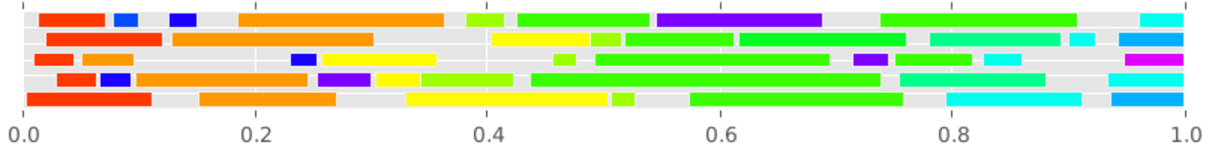
\includegraphics[width=\textwidth]{act_gt_2}
      \caption*{Ground Truth Activity Labels}
    \end{subfigure}
    \begin{subfigure}[b]{\textwidth}
      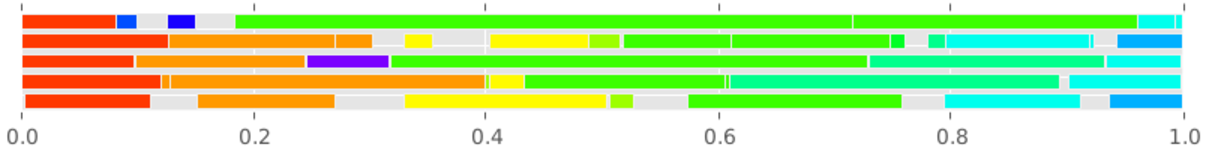
\includegraphics[width=\textwidth]{act_our_2}
      \caption*{Activity Labels extracted by Our Method}
    \end{subfigure}
    \begin{subfigure}[b]{0.5\textwidth}
      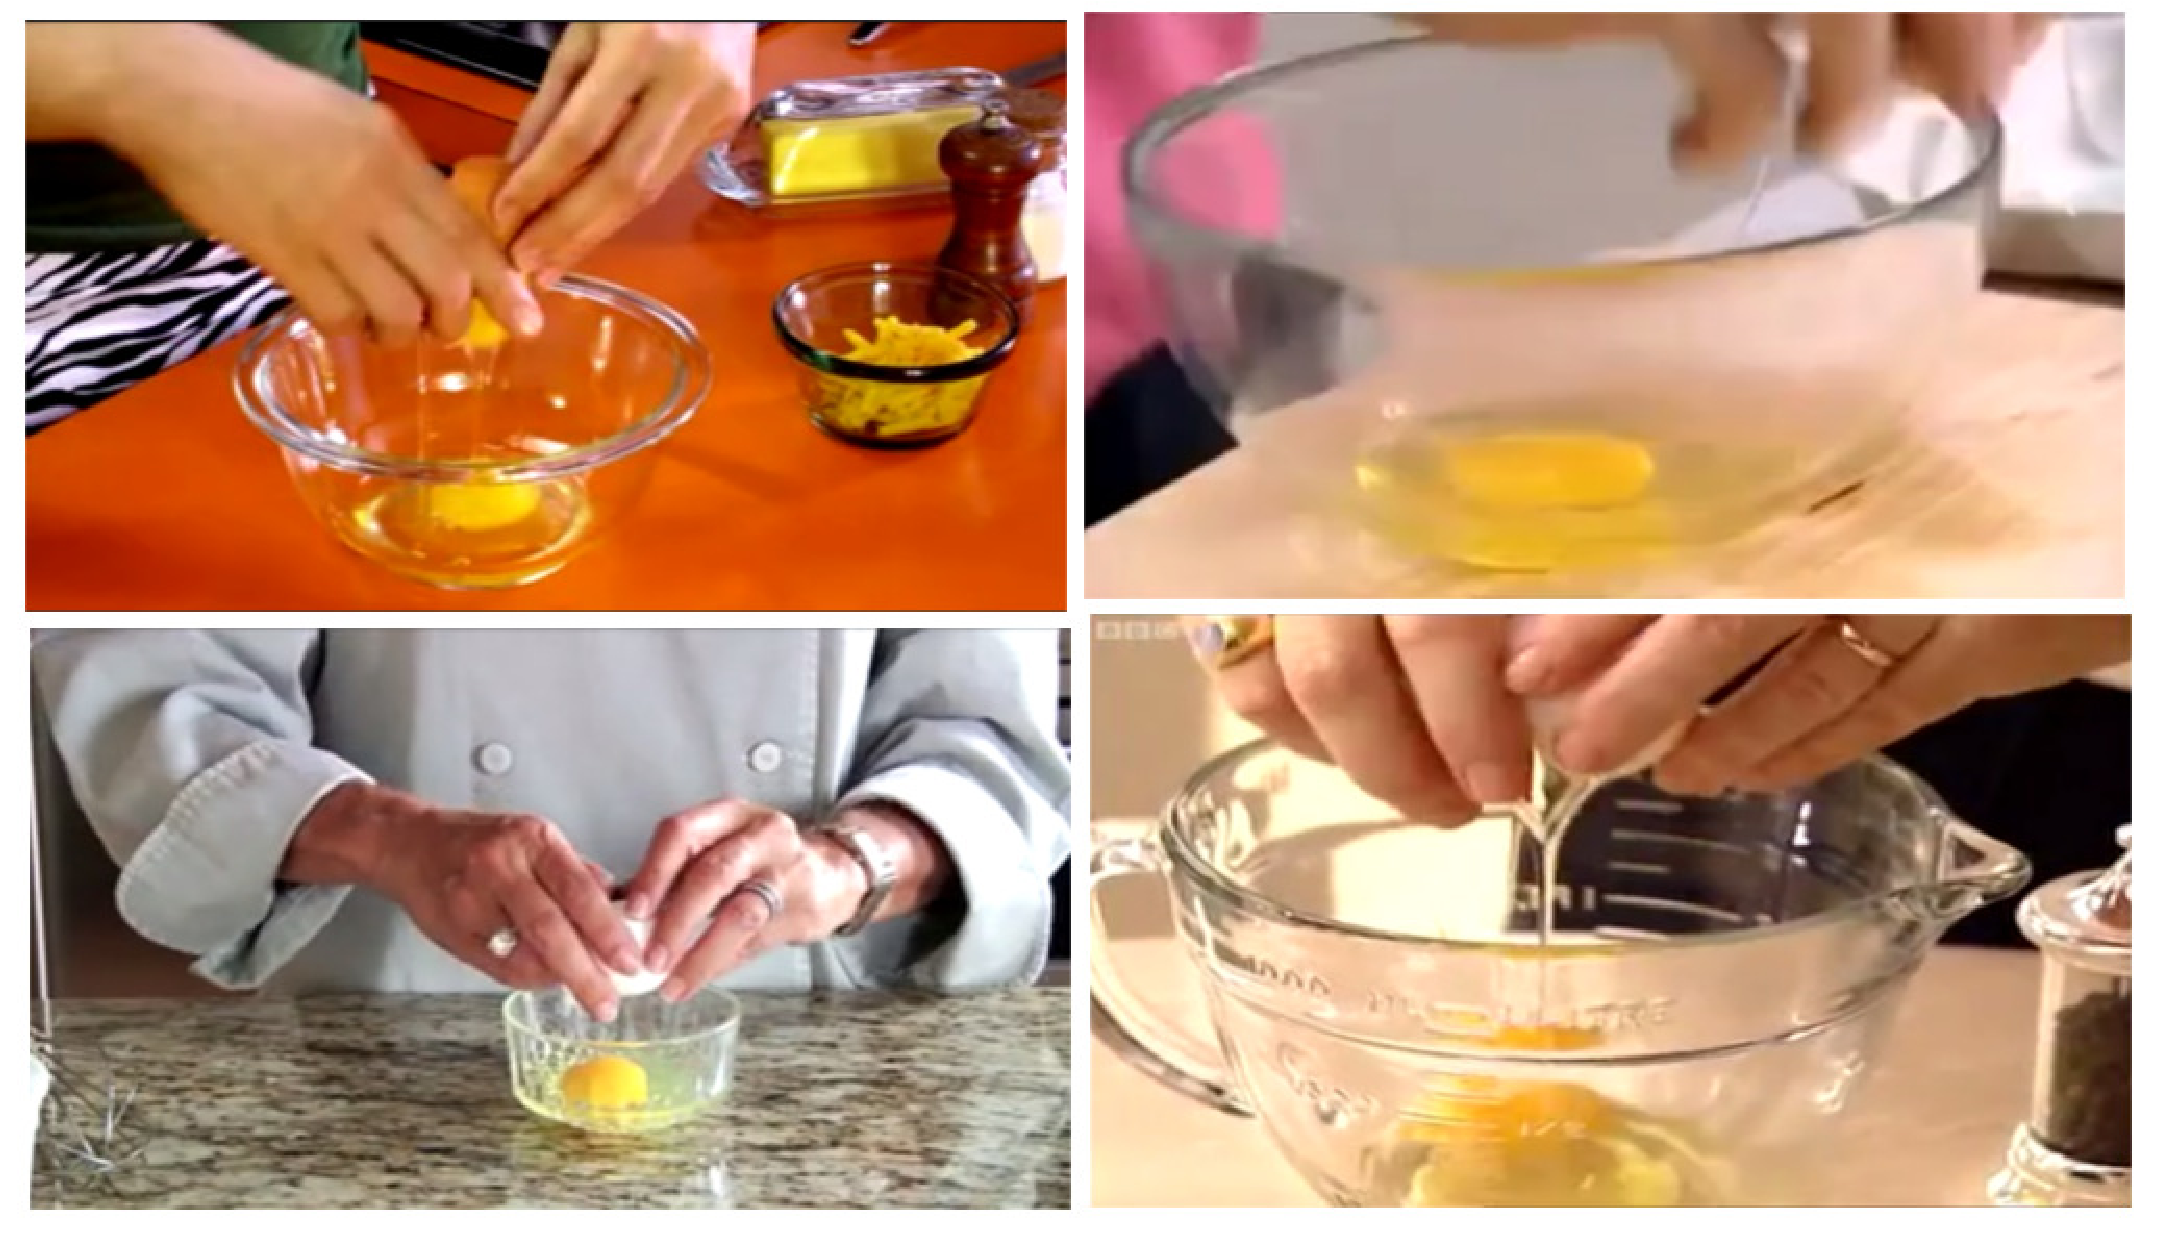
\includegraphics[width=\textwidth]{cred}
      \color[HTML]{FF3800}{Crack the eggs one at a time into a bowl.}
    \end{subfigure}~
    \begin{subfigure}[b]{0.5\textwidth}
      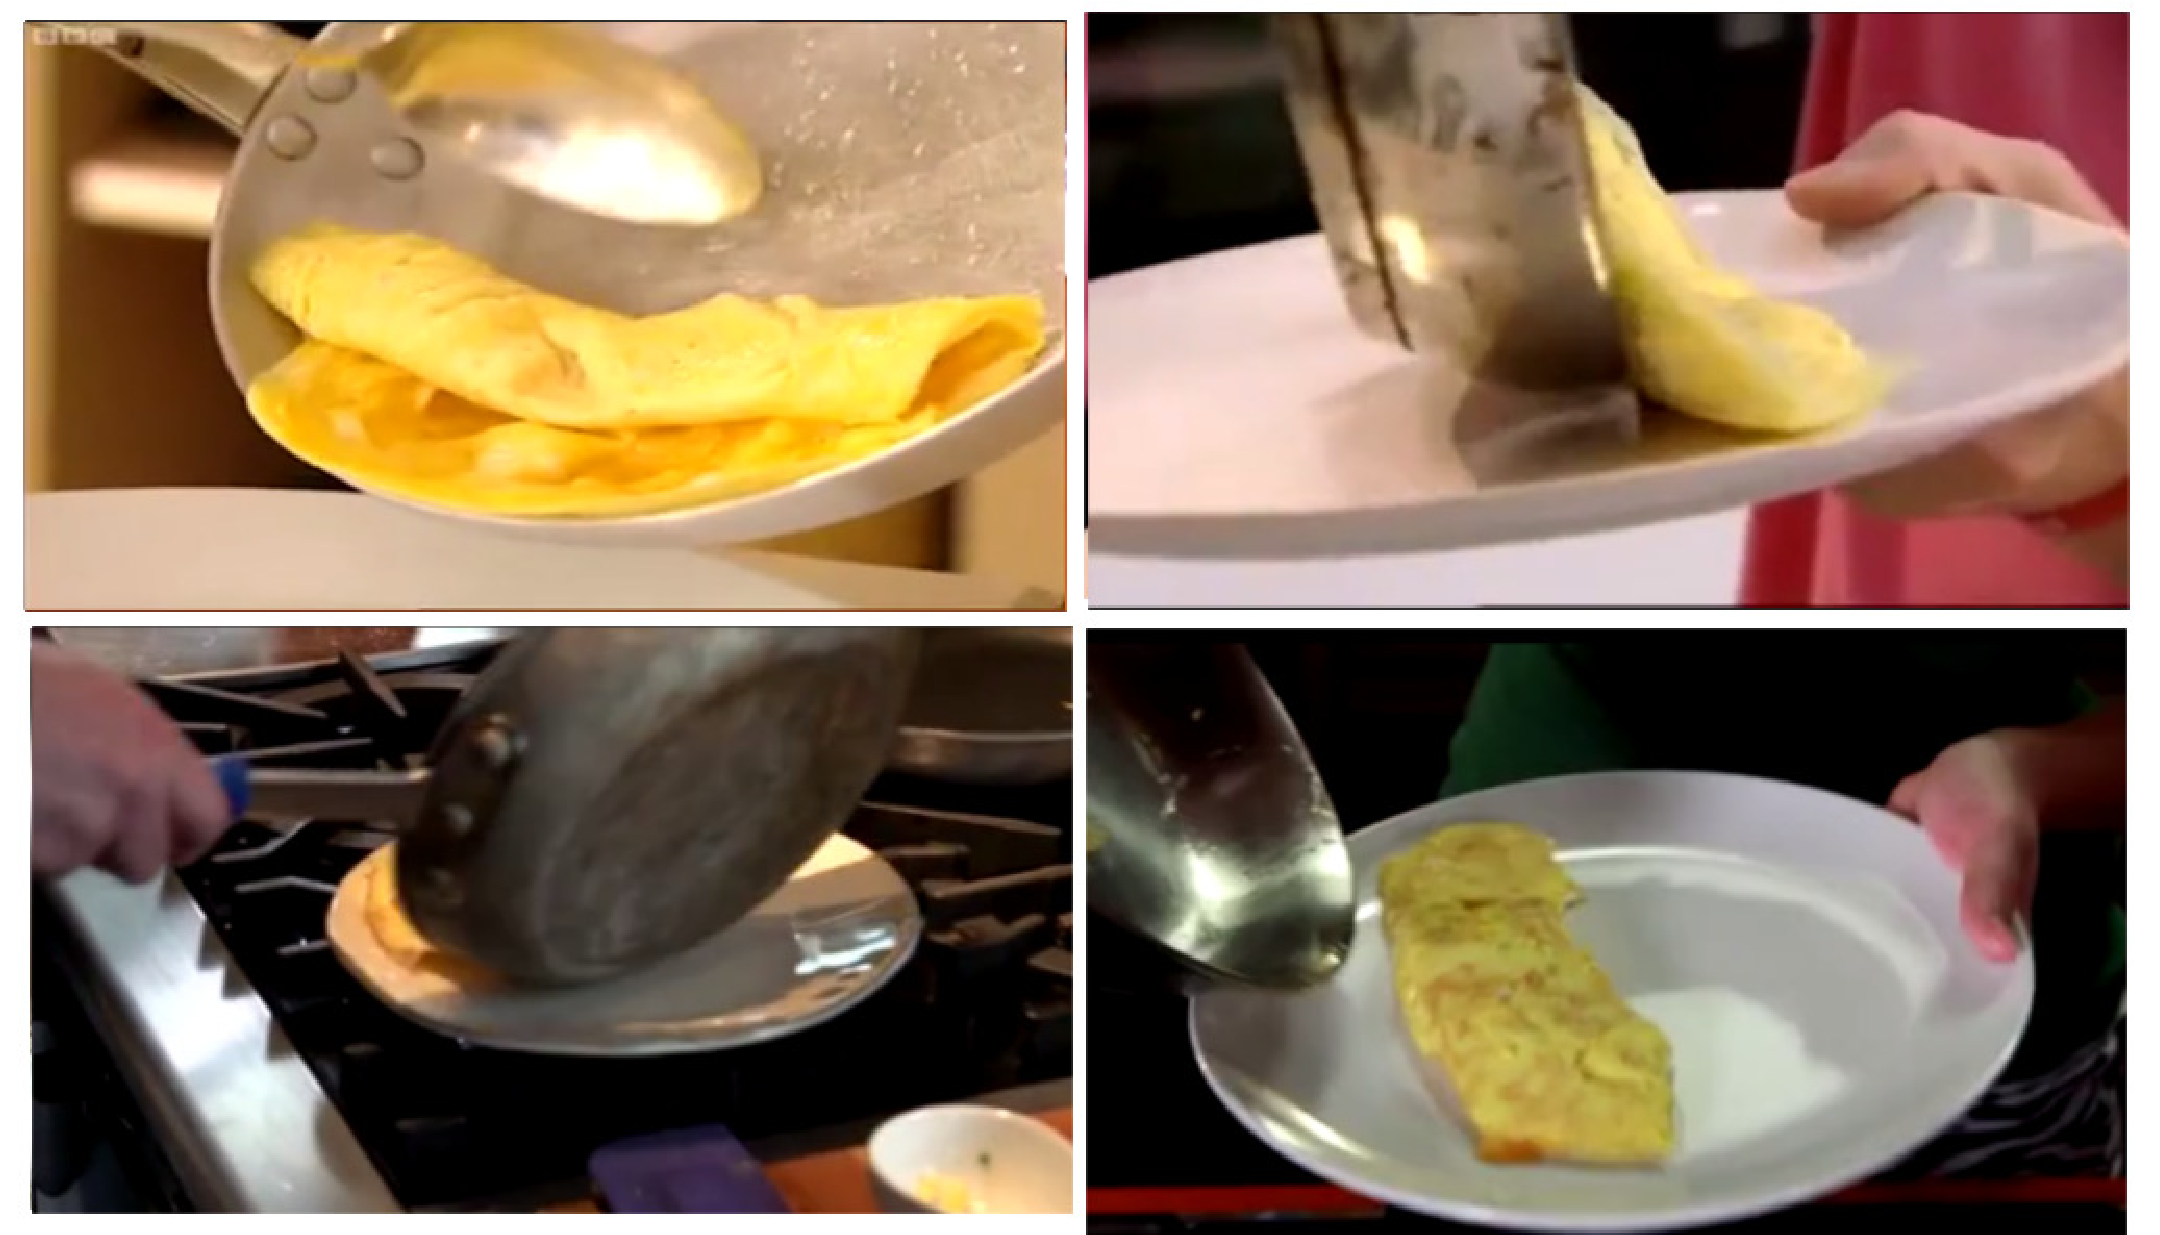
\includegraphics[width=\textwidth]{cyan}
      \color[HTML]{00FFED}{Remove the omelette onto a plate.}
    \end{subfigure}
    \begin{subfigure}[b]{0.5\textwidth}
      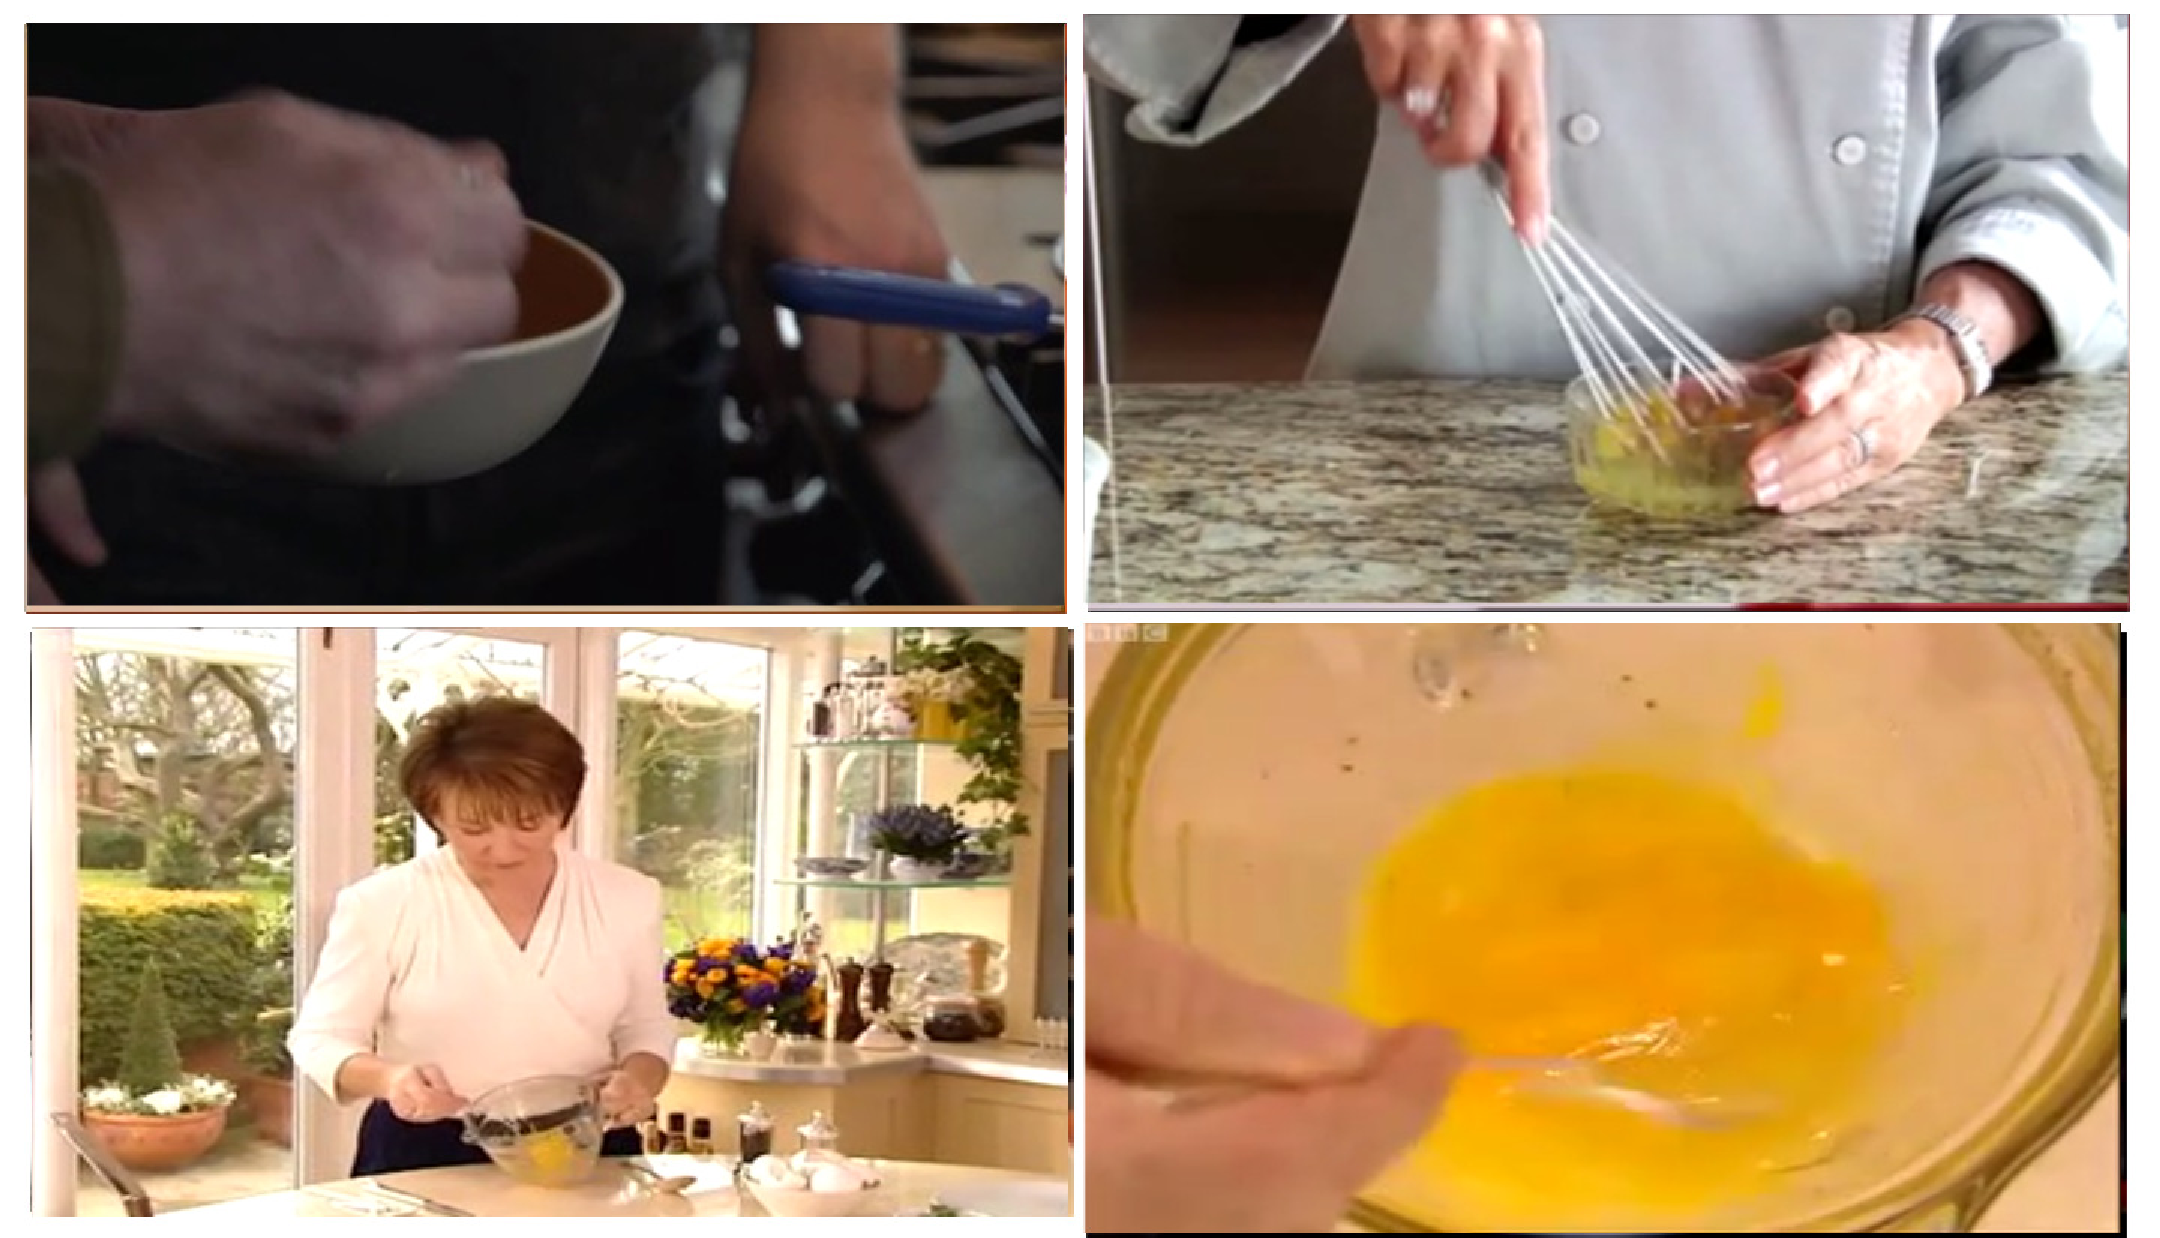
\includegraphics[width=\textwidth]{corange}
      \color[HTML]{FF9900}{You can either use a fork or wire whisk to beat the eggs into a bowl.}
    \end{subfigure}~
    \begin{subfigure}[b]{0.5\textwidth}
      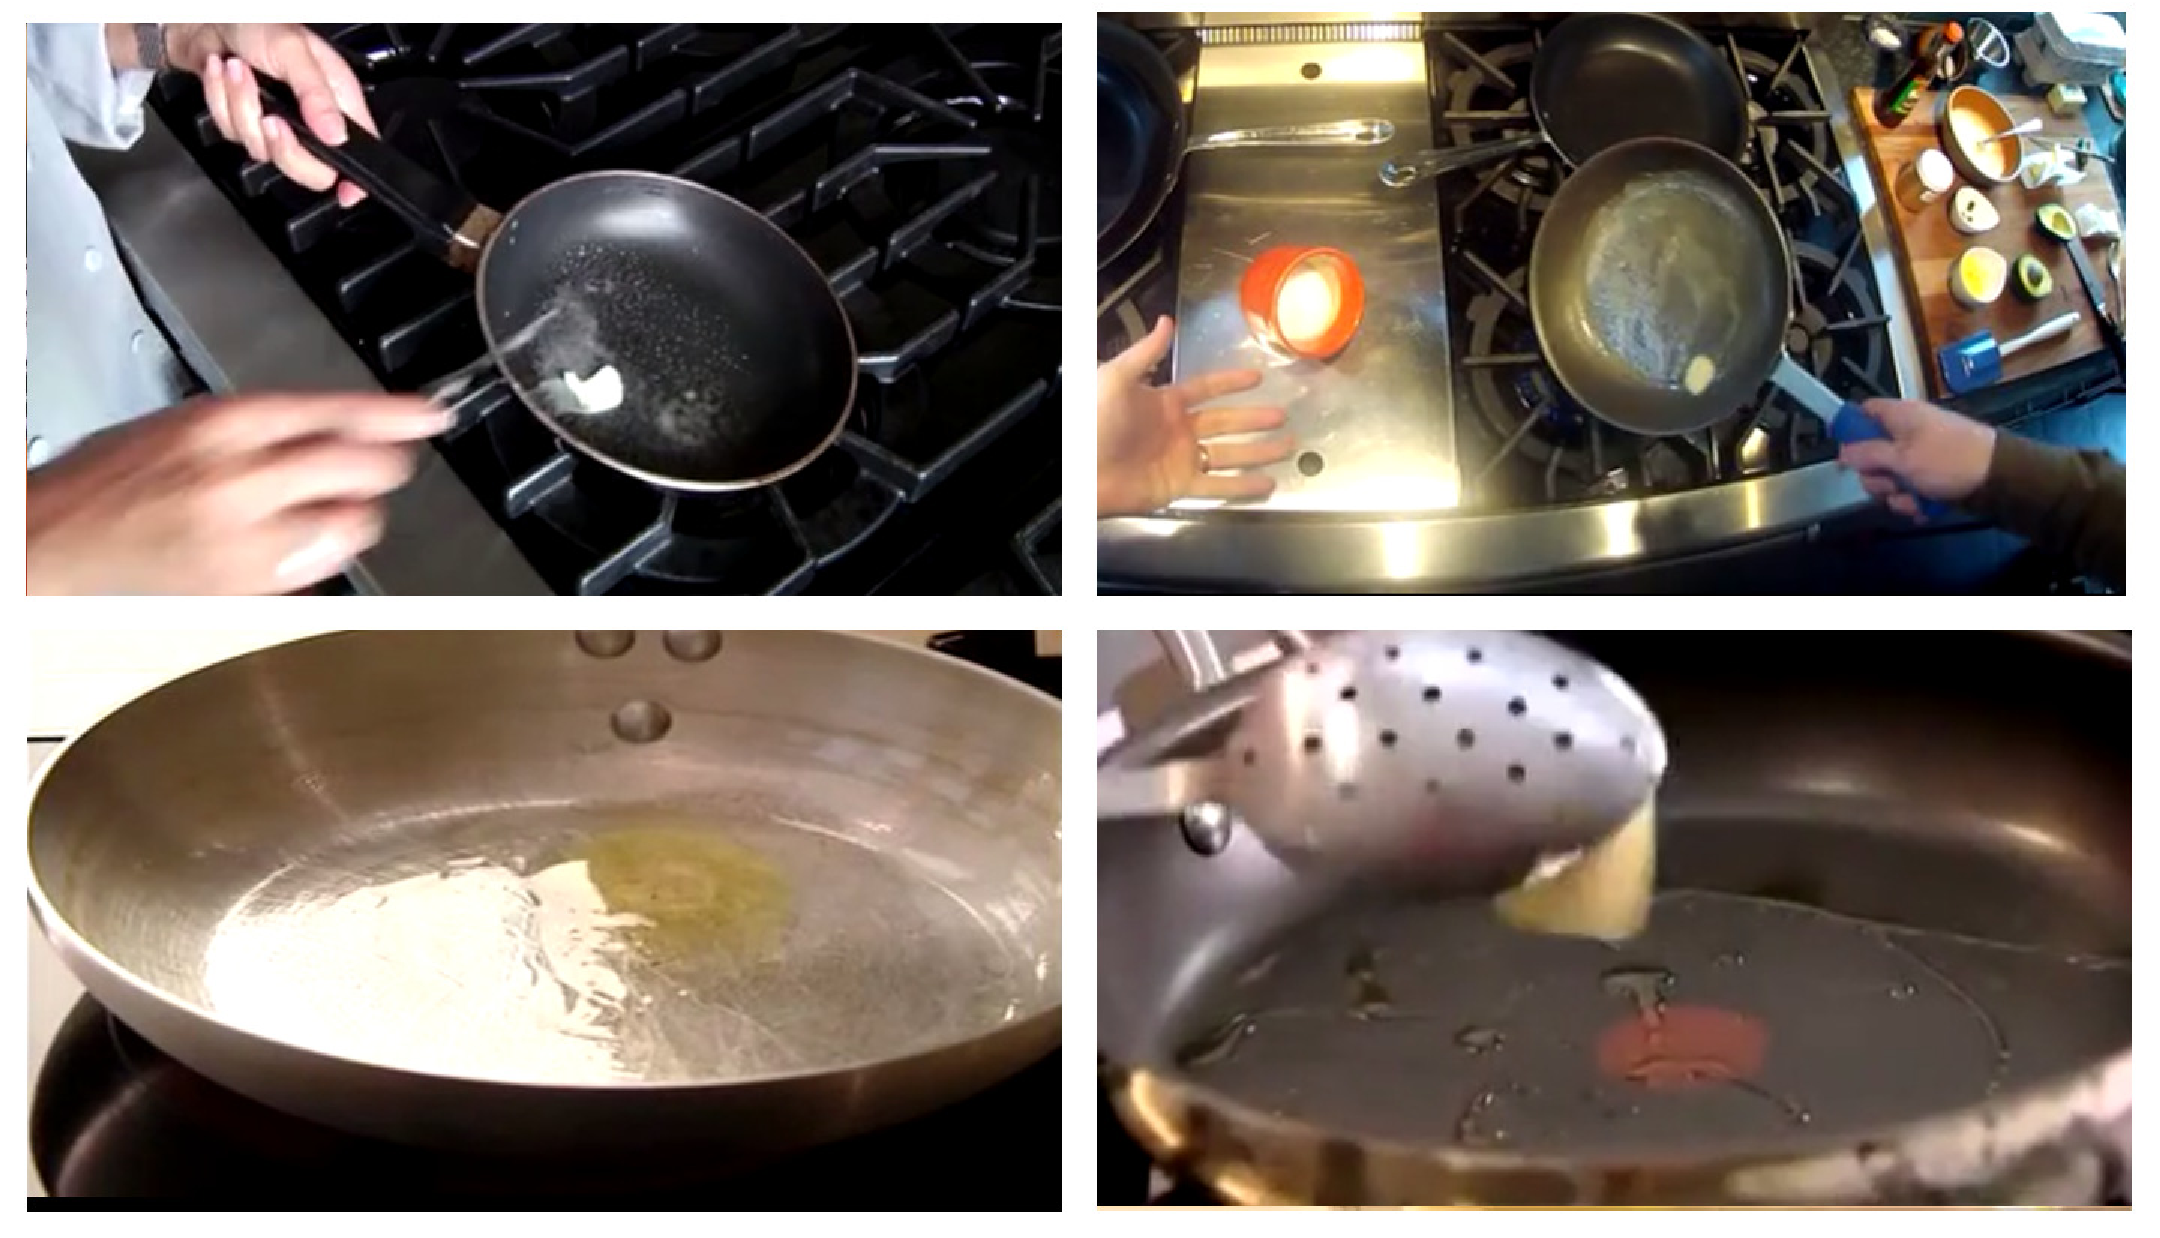
\includegraphics[width=\textwidth]{cgreen}
      \color[HTML]{9DFF00}{Eggs cook quickly, so make sure the pan gets very hot first; the butter melt completely.}
    \end{subfigure}
    \caption{How to make an ommelette?}
  \end{subfigure}\quad\quad\begin{subfigure}[b]{0.47\textwidth}
    \begin{subfigure}[b]{\textwidth}
      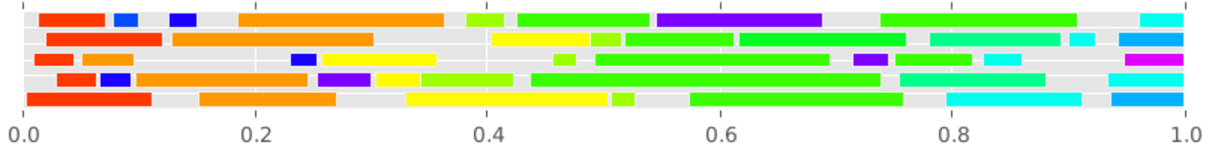
\includegraphics[width=\textwidth]{act_gt_2}
      \caption*{Ground Truth Activity Labels}
    \end{subfigure}
    \begin{subfigure}[b]{\textwidth}
      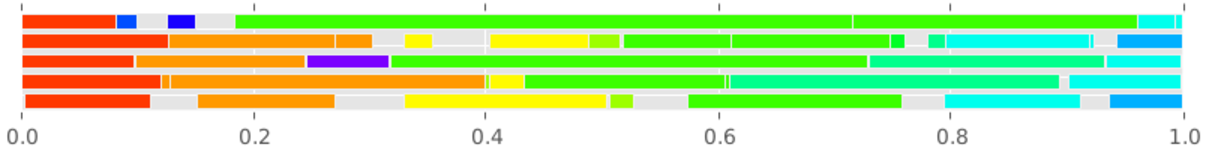
\includegraphics[width=\textwidth]{act_our_2}
      \caption*{Activity Labels extracted by Our Method}
    \end{subfigure}
    \begin{subfigure}[b]{0.5\textwidth}
      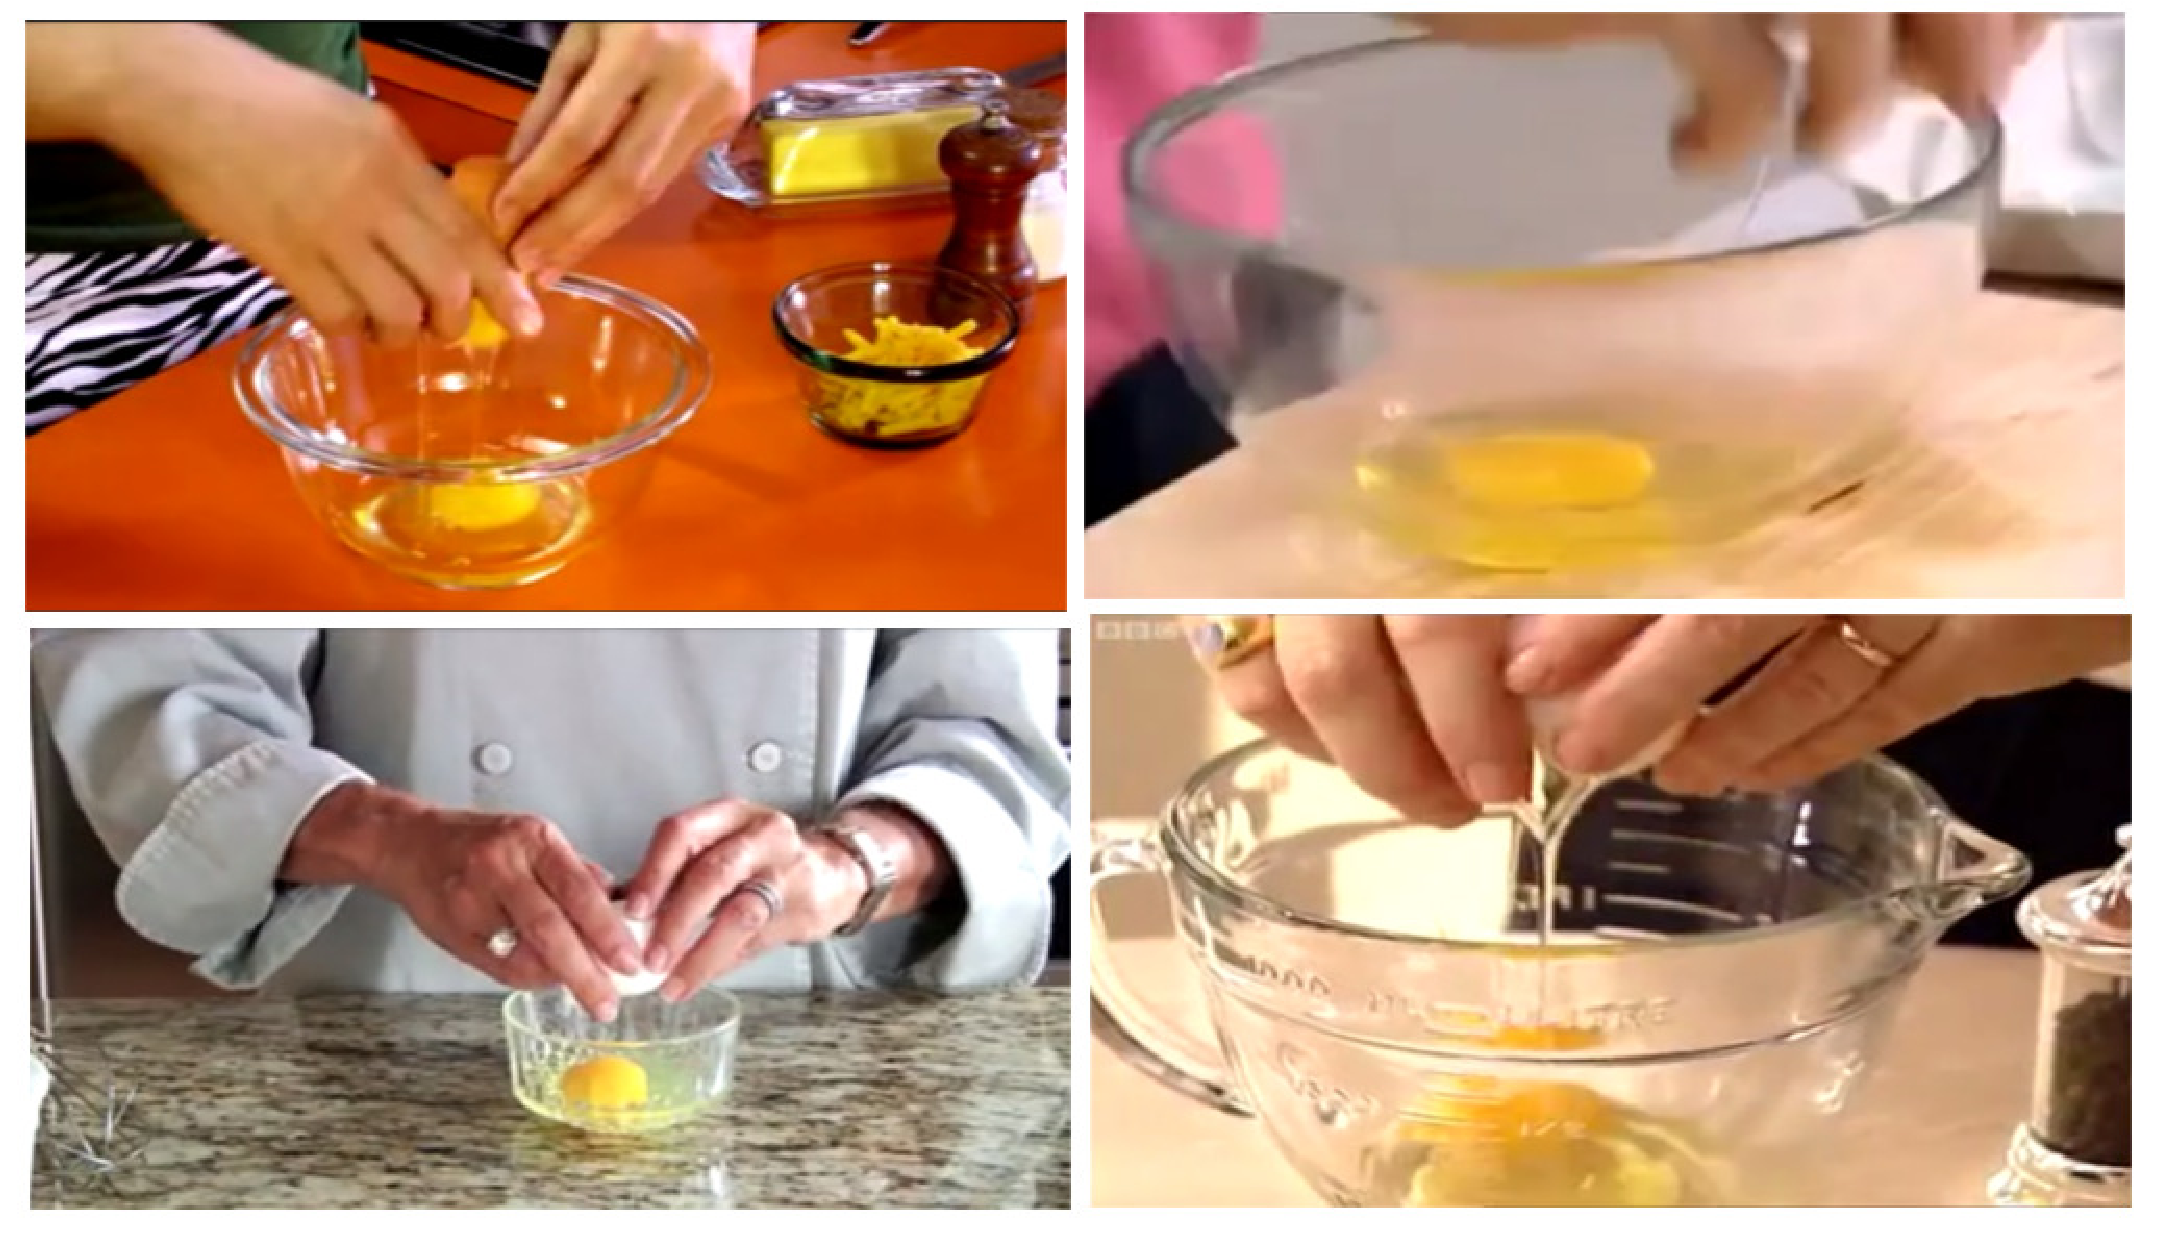
\includegraphics[width=\textwidth]{cred}
      \color[HTML]{FF3800}{Crack the eggs one at a time into a bowl.}
    \end{subfigure}~
    \begin{subfigure}[b]{0.5\textwidth}
      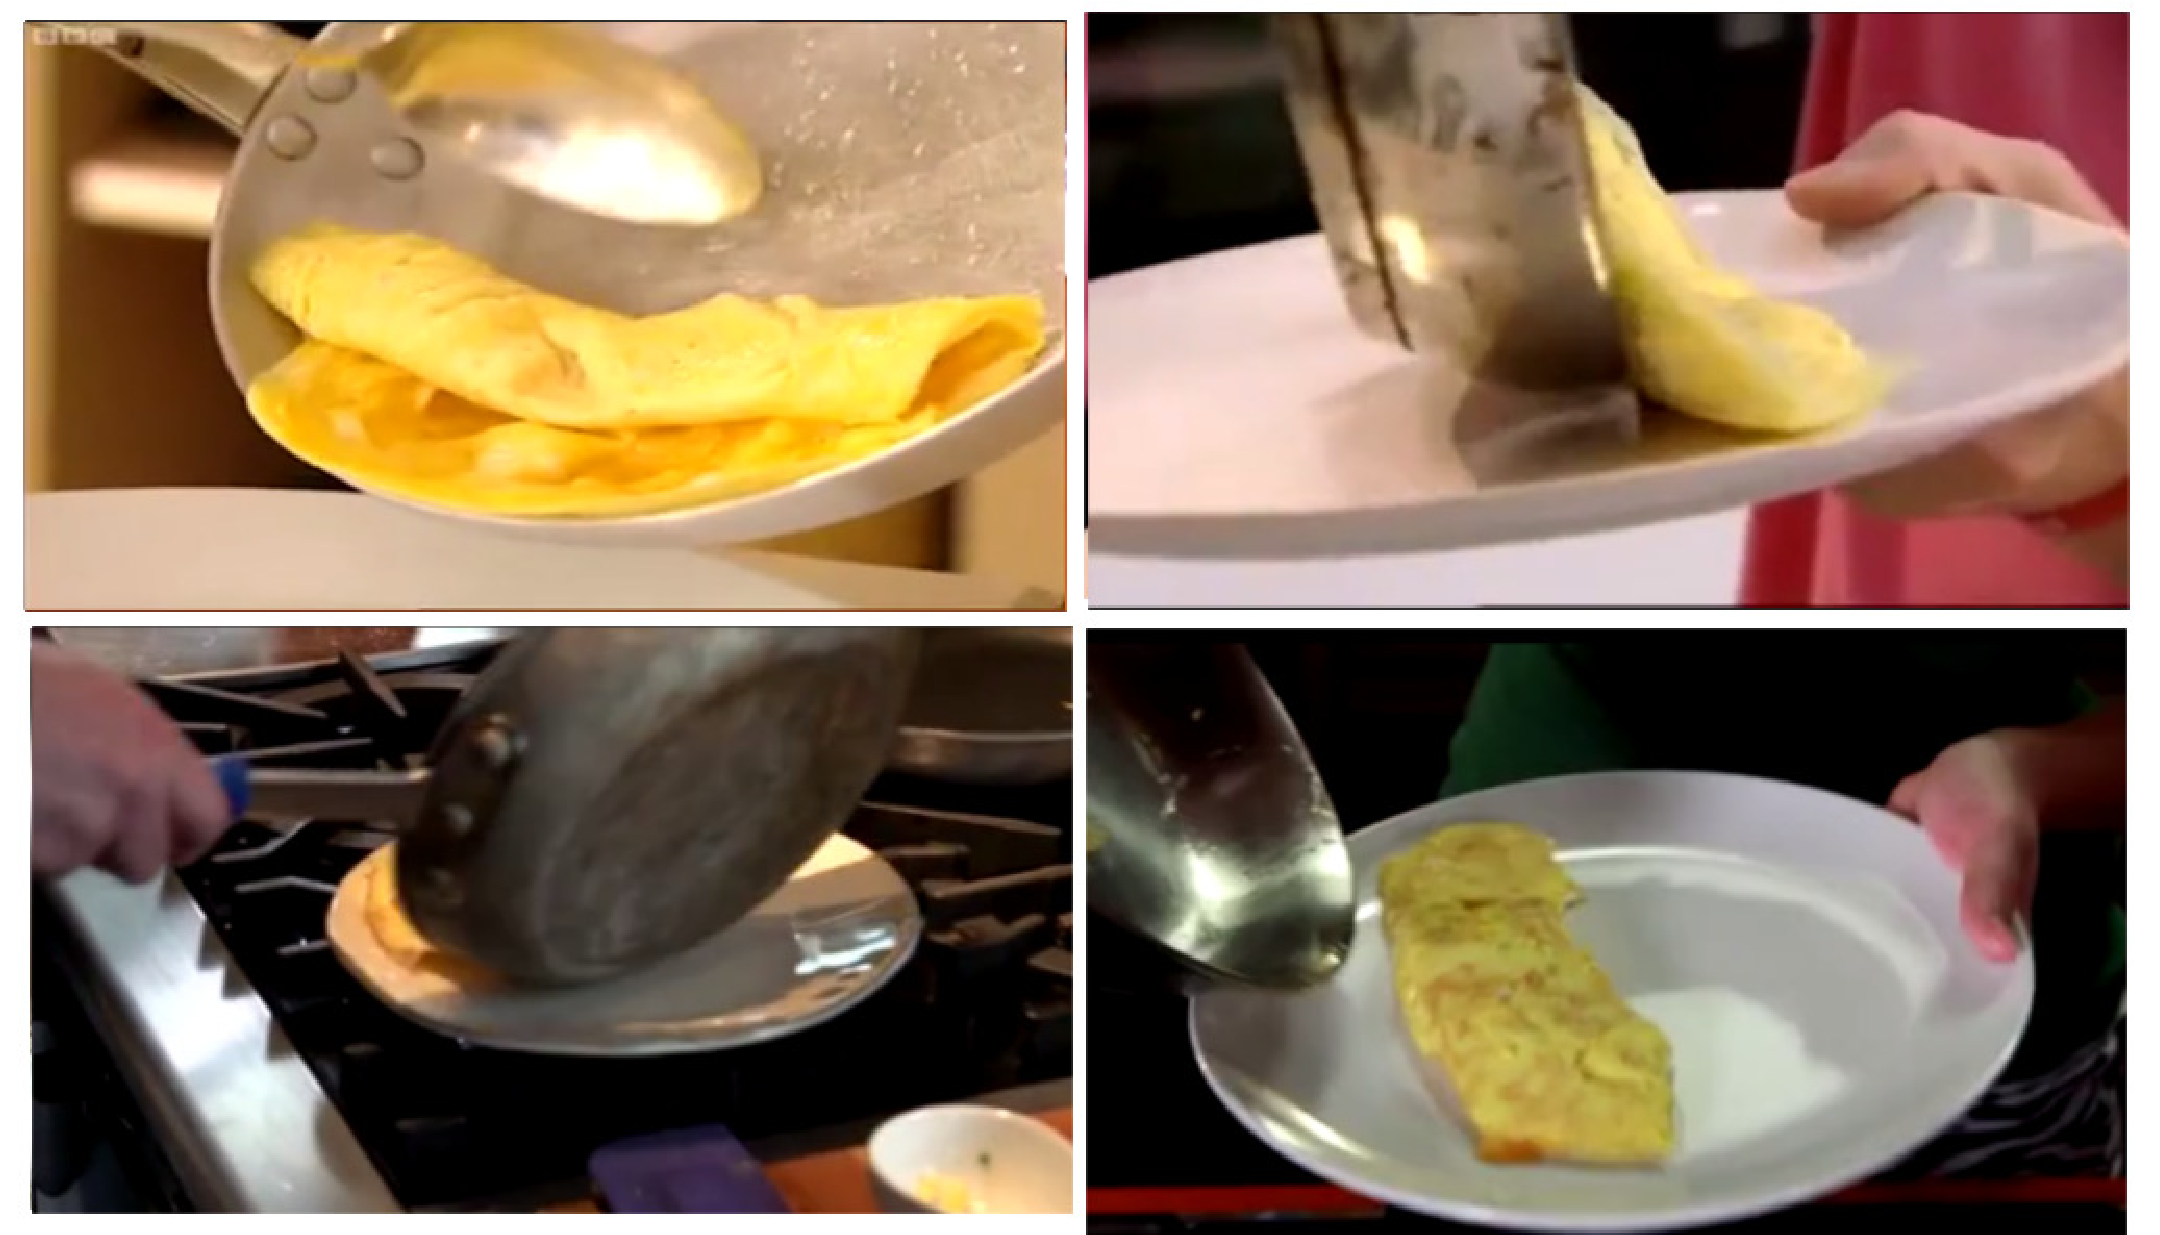
\includegraphics[width=\textwidth]{cyan}
      \color[HTML]{00FFED}{Remove the omelette onto a plate.}
    \end{subfigure}
    \begin{subfigure}[b]{0.5\textwidth}
      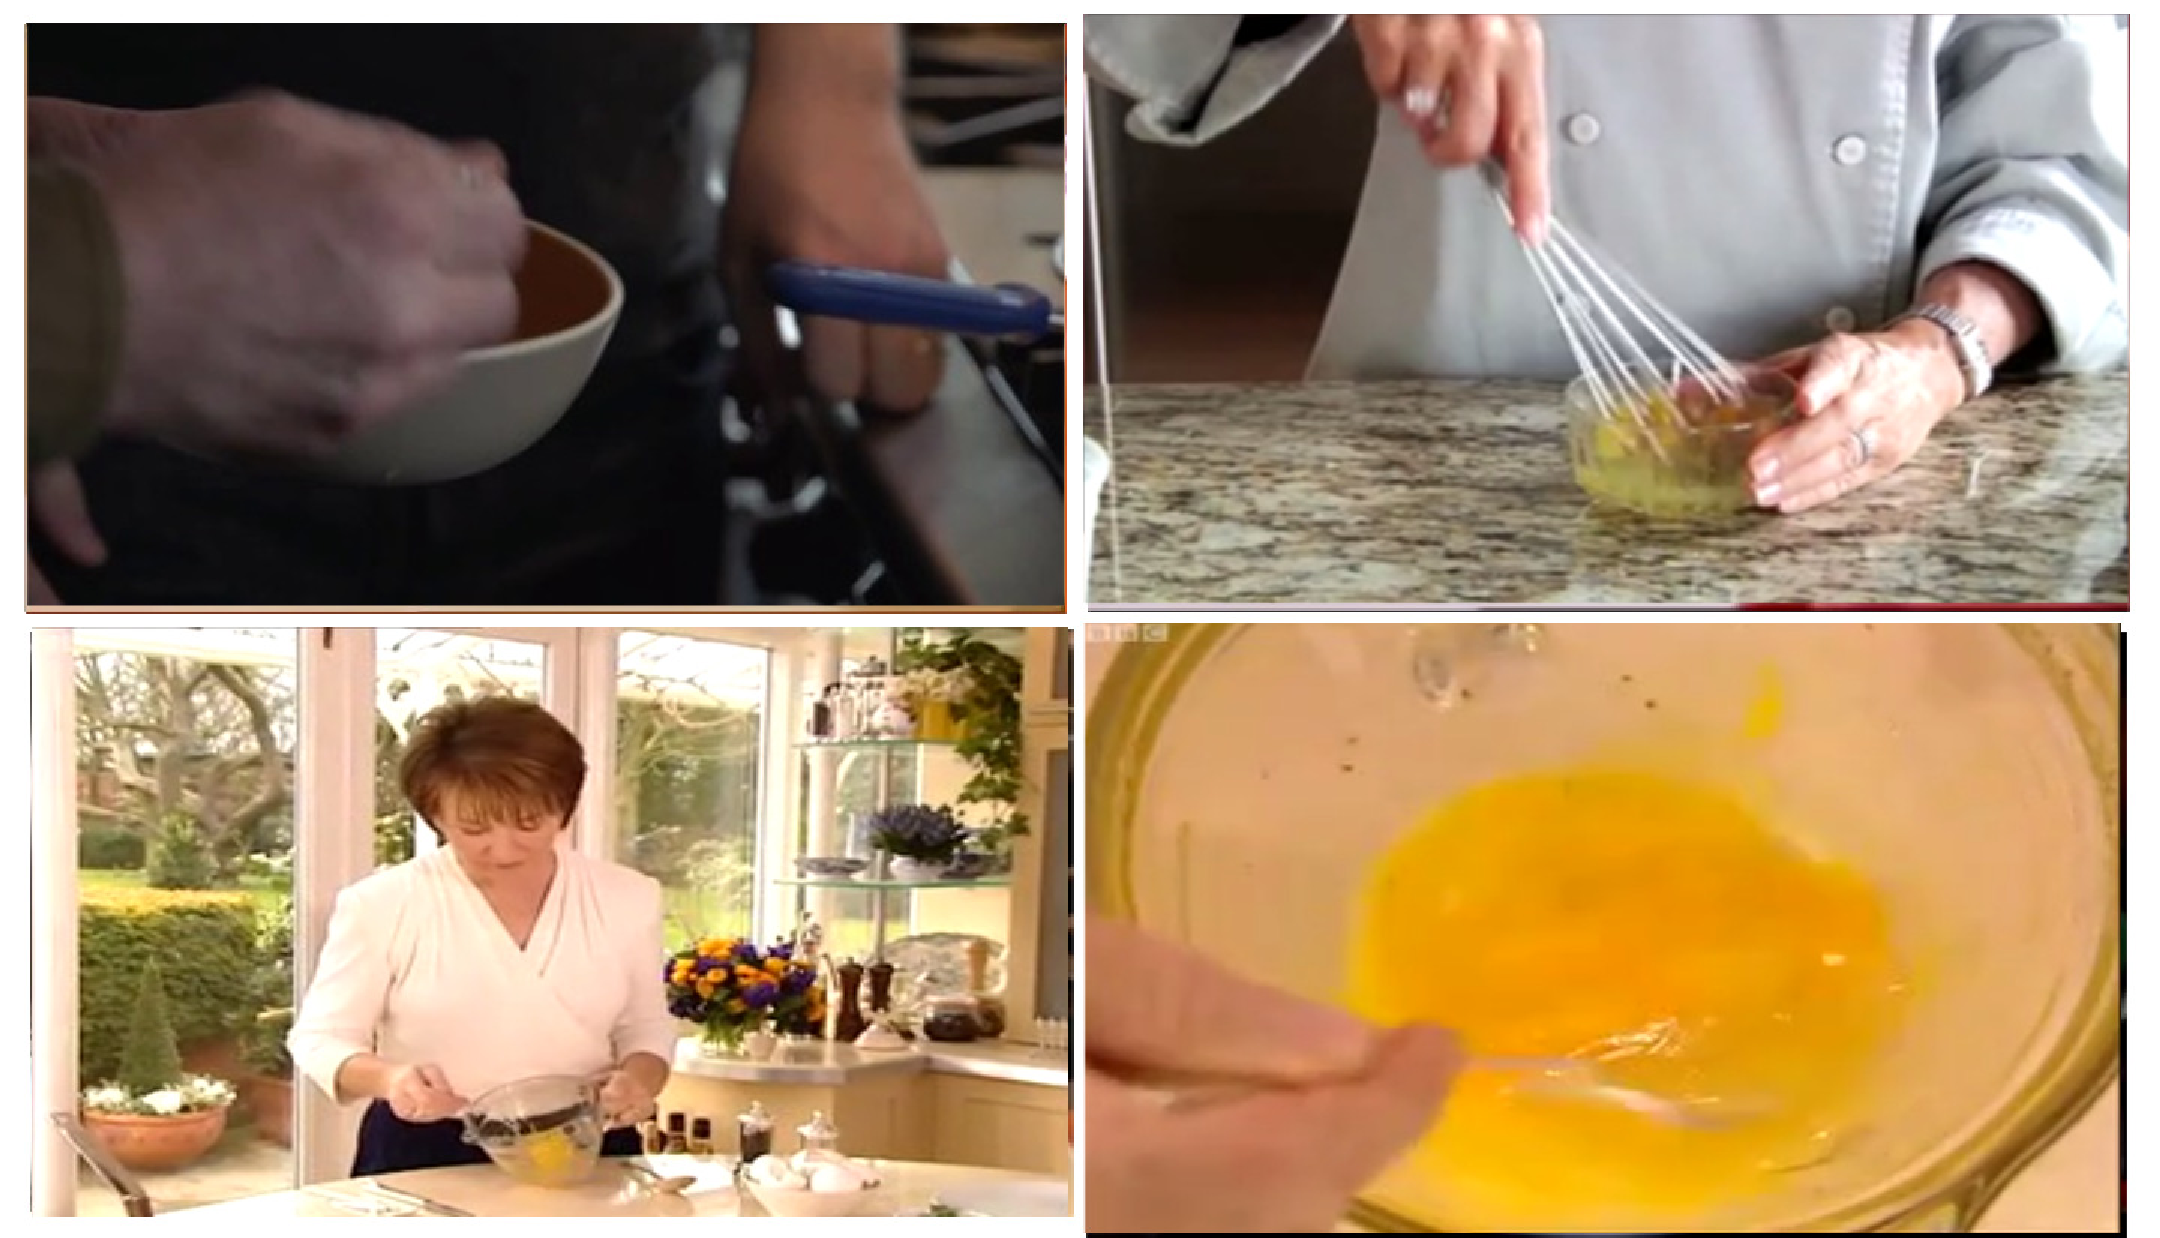
\includegraphics[width=\textwidth]{corange}
      \color[HTML]{FF9900}{You can either use a fork or wire whisk to beat the eggs into a bowl.}
    \end{subfigure}~
    \begin{subfigure}[b]{0.5\textwidth}
      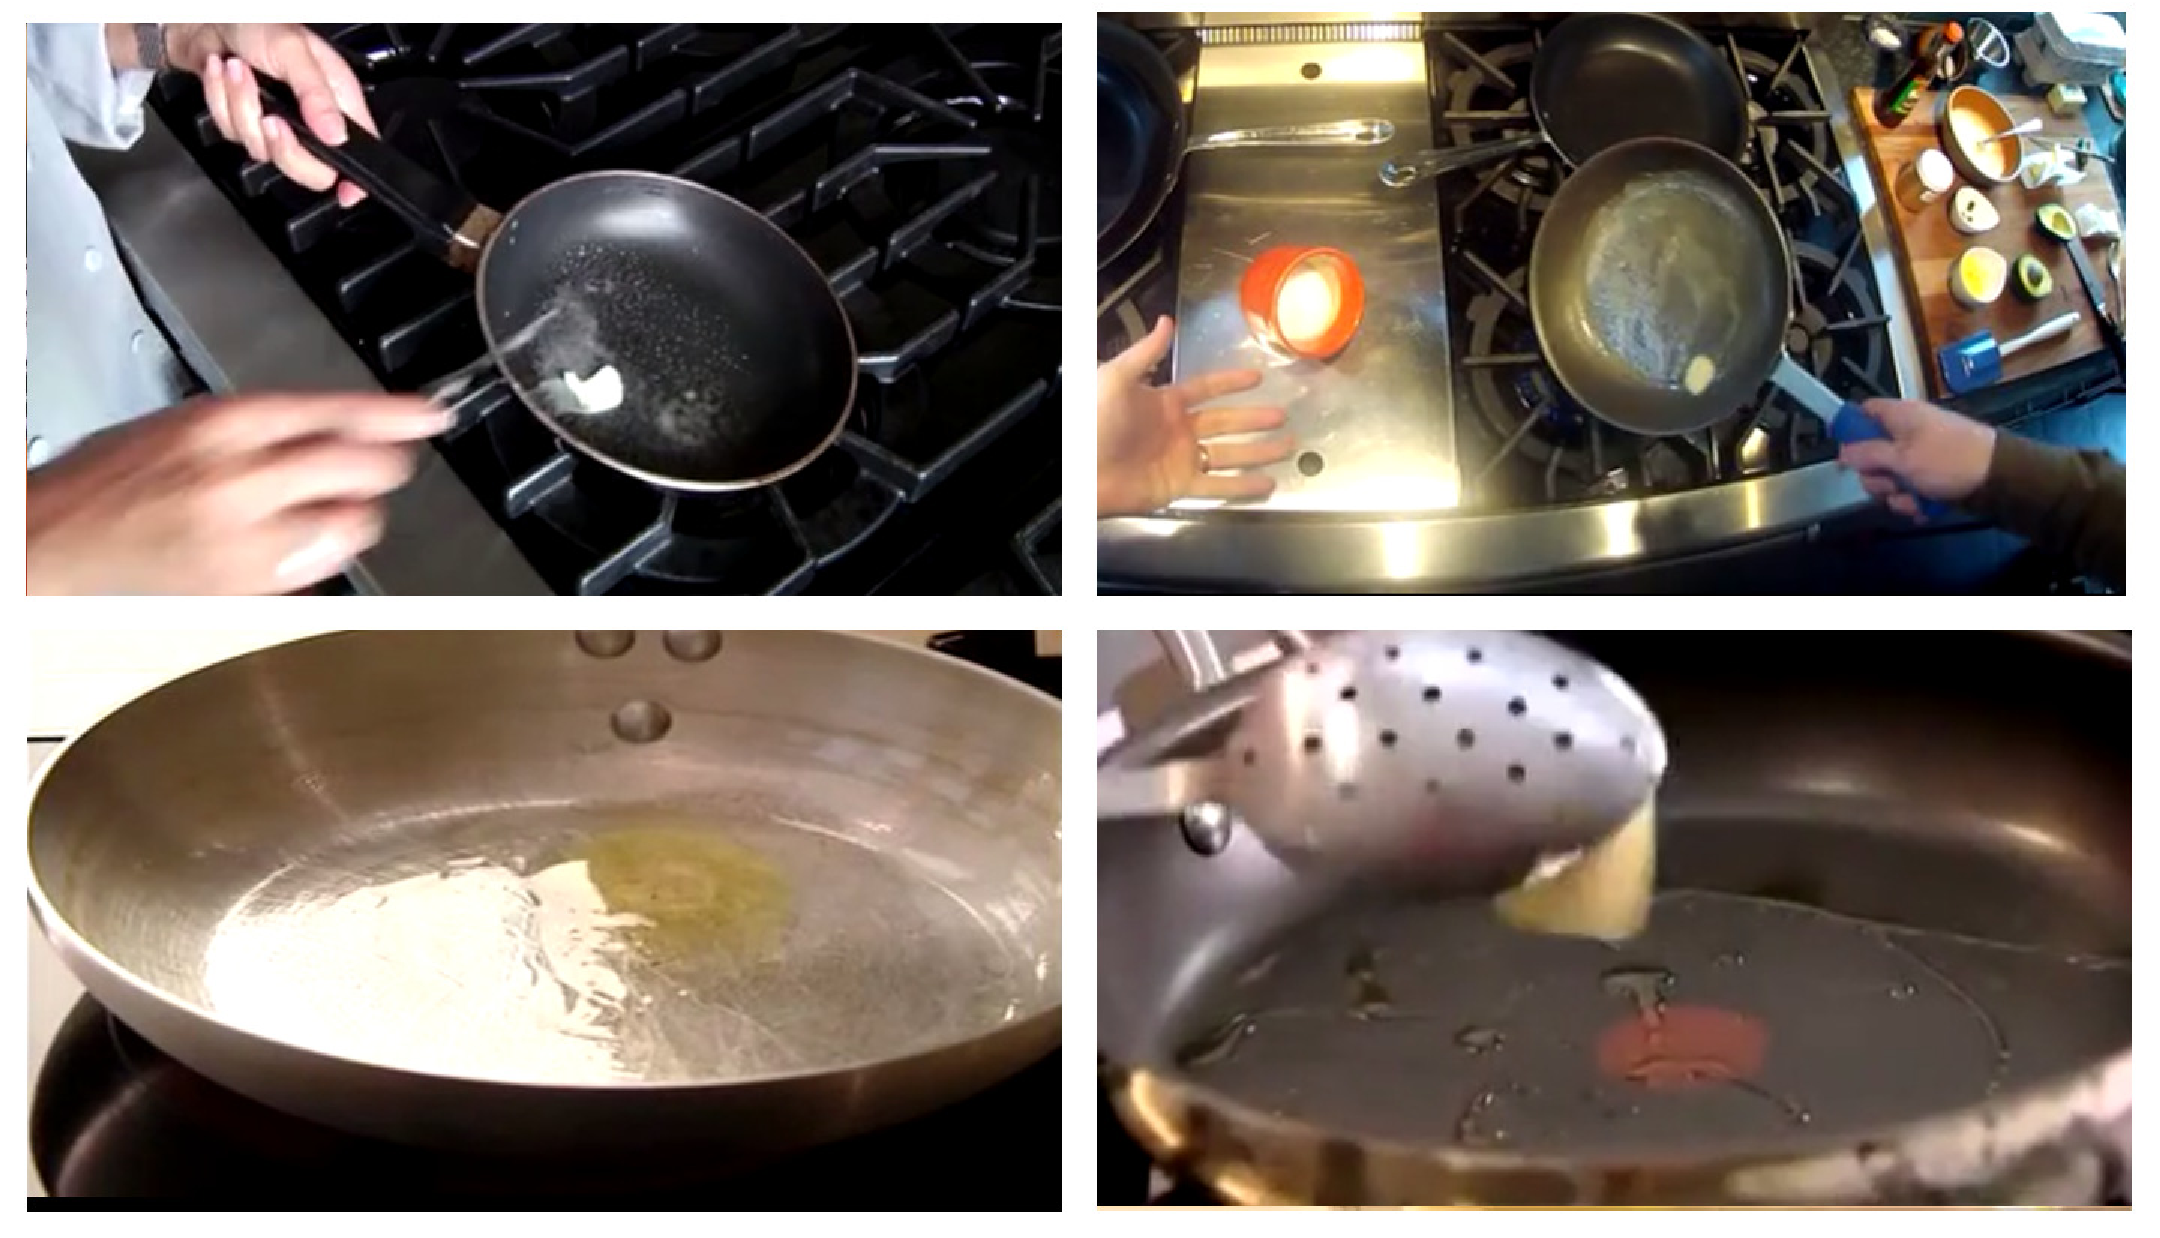
\includegraphics[width=\textwidth]{cgreen}
      \color[HTML]{9DFF00}{Eggs cook quickly, so make sure the pan gets very hot first; the butter melt completely.}
    \end{subfigure}
    \caption{How to make a milkshake?}
  \end{subfigure}
\caption{Temporal segmentation of the videos by our method and ground truth segmentation. We also color code the learned activity labels and visualize sample frames and the automatically generated captions for some of them. \emph{Best viewed in color.}}
\label{recipe:ommelette}
\iffalse
\begin{subfigure}[b]{0.5\textwidth}
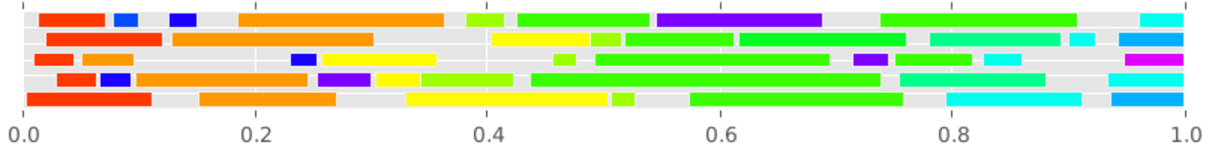
\includegraphics[width=\textwidth]{act_gt_2}
\caption{Ground Truth Activity Labels}
\end{subfigure}
\begin{subfigure}[b]{0.5\textwidth}
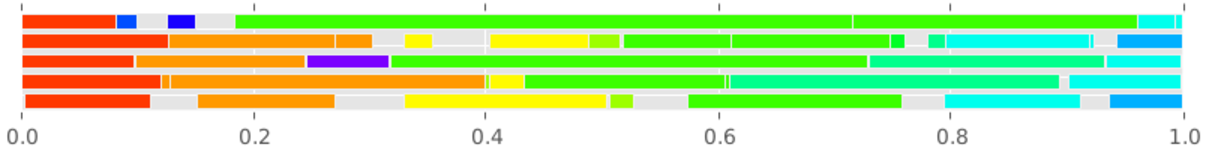
\includegraphics[width=\textwidth]{act_our_2}
\caption{Activity Labels extracted by Our Method}
\end{subfigure}
\begin{subfigure}[b]{0.25\textwidth}
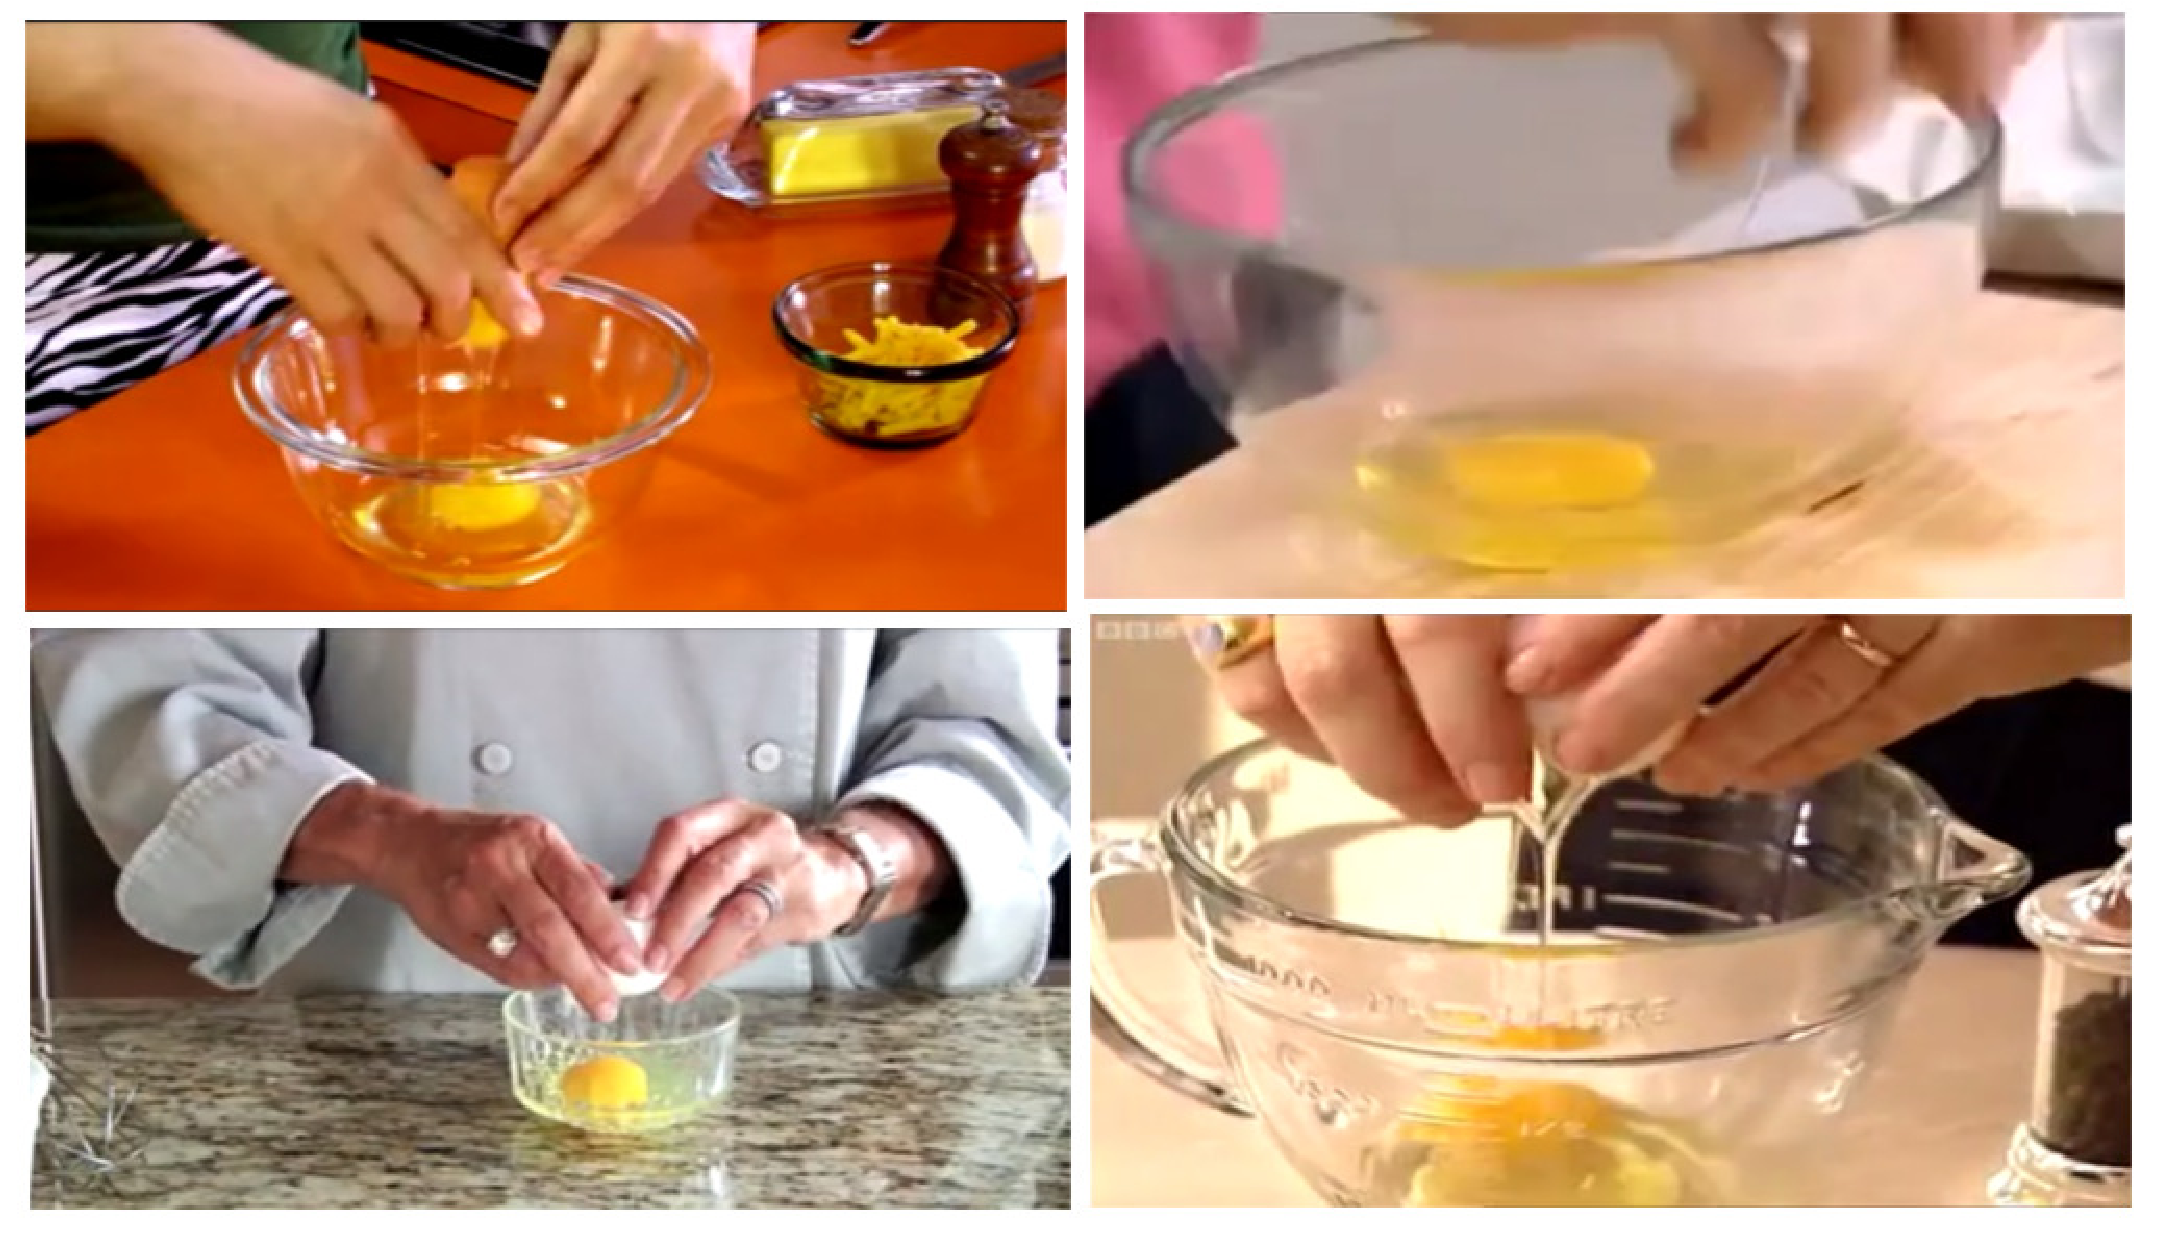
\includegraphics[width=\textwidth]{cred}
\color[HTML]{FF3800}{Crack the eggs one at a time into a bowl.}
\end{subfigure}~
\begin{subfigure}[b]{0.25\textwidth}
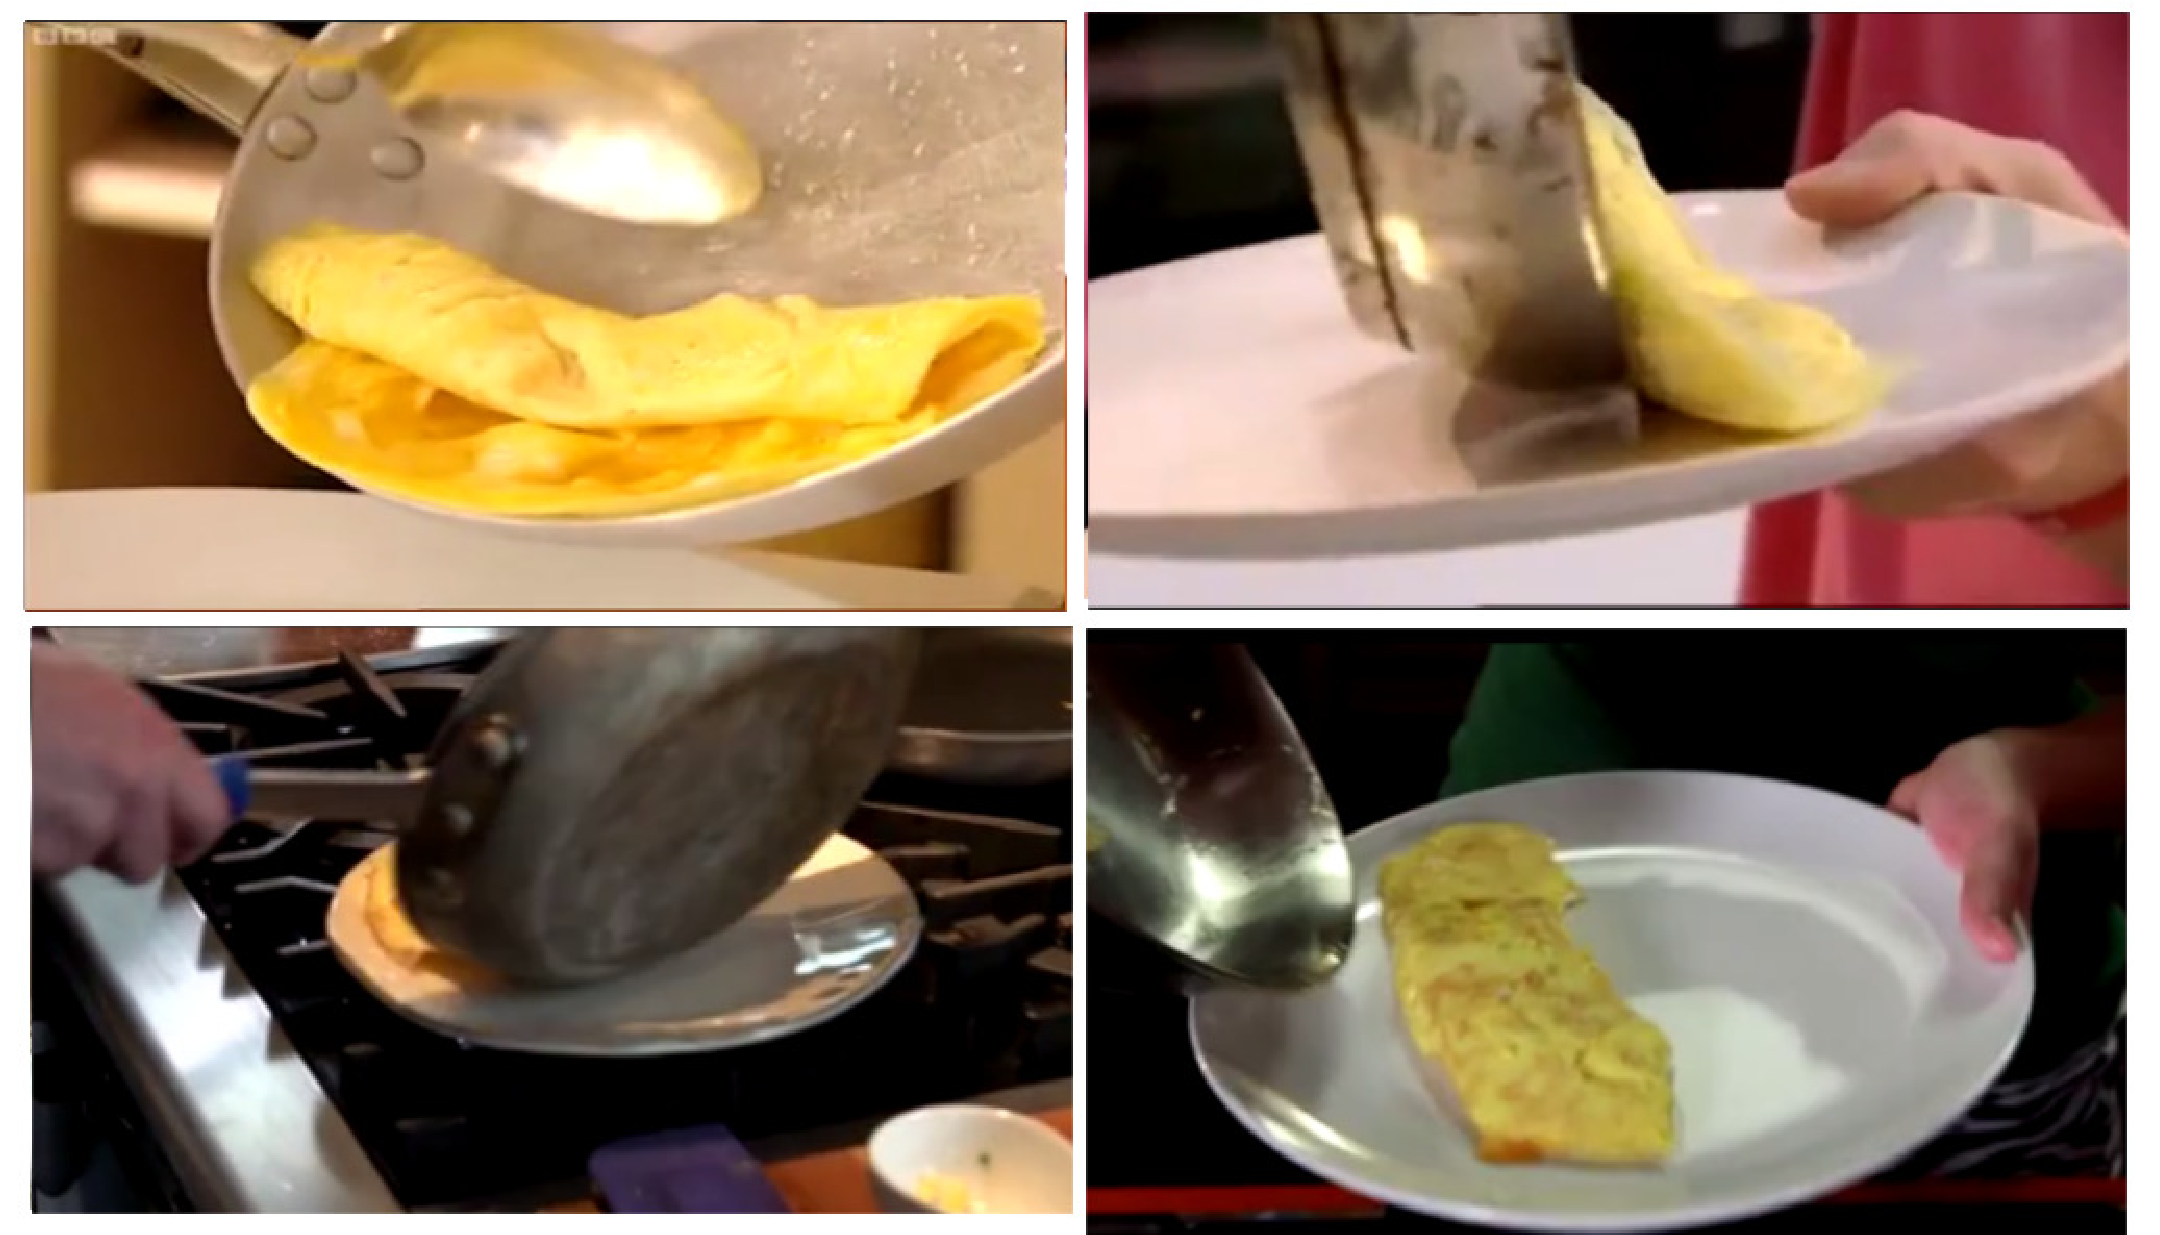
\includegraphics[width=\textwidth]{cyan}
\color[HTML]{00FFED}{Remove the omelette onto a plate.}
\end{subfigure}
\begin{subfigure}[b]{0.25\textwidth}
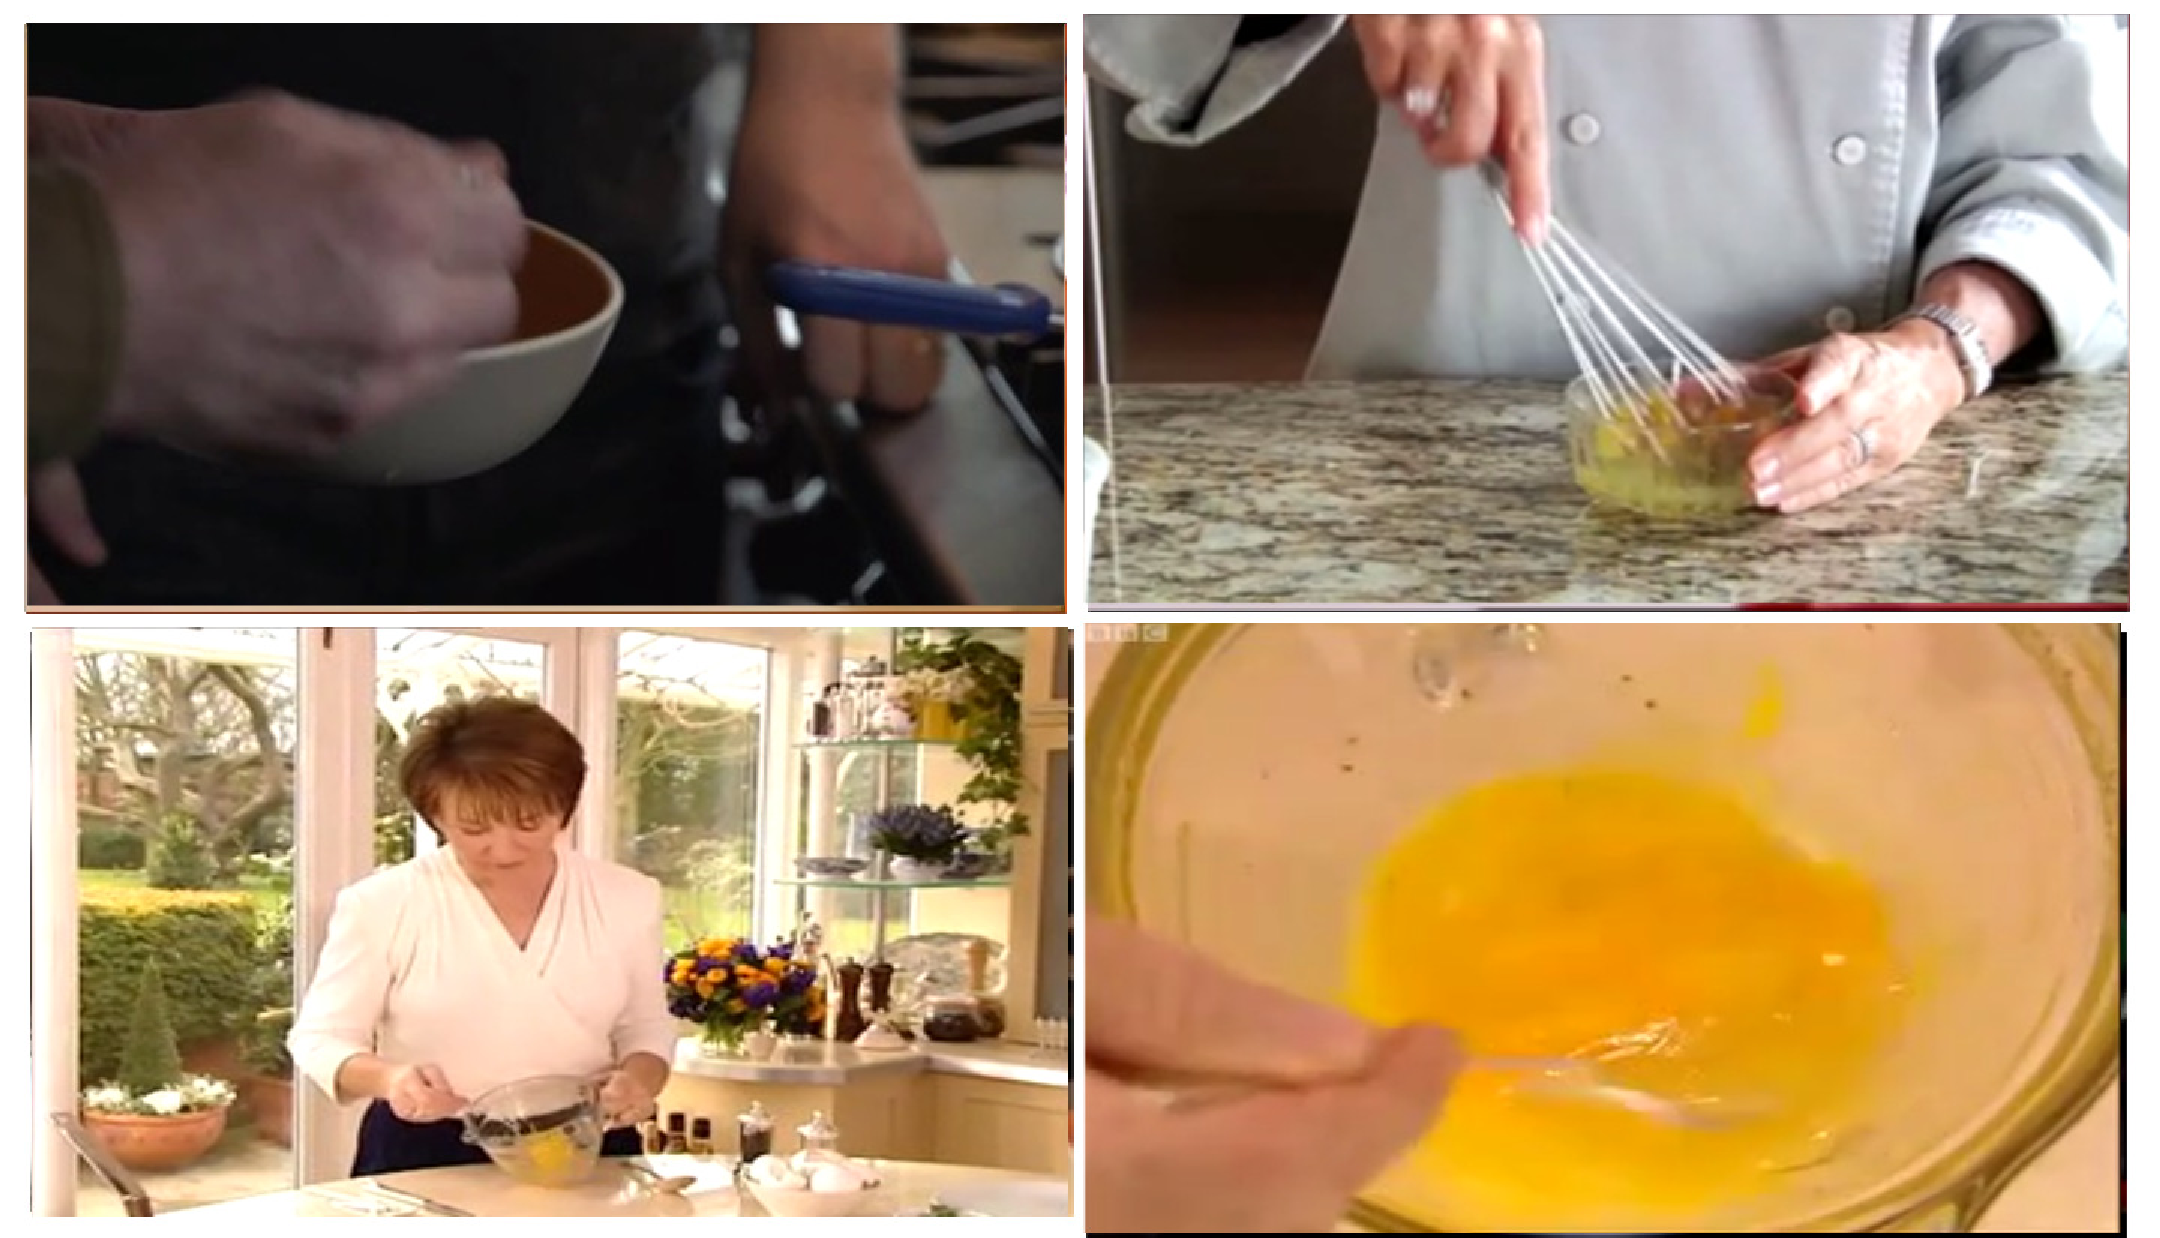
\includegraphics[width=\textwidth]{corange}
\color[HTML]{FF9900}{You can either use a fork or wire whisk to beat the eggs into a bowl.}
\end{subfigure}~
\begin{subfigure}[b]{0.25\textwidth}
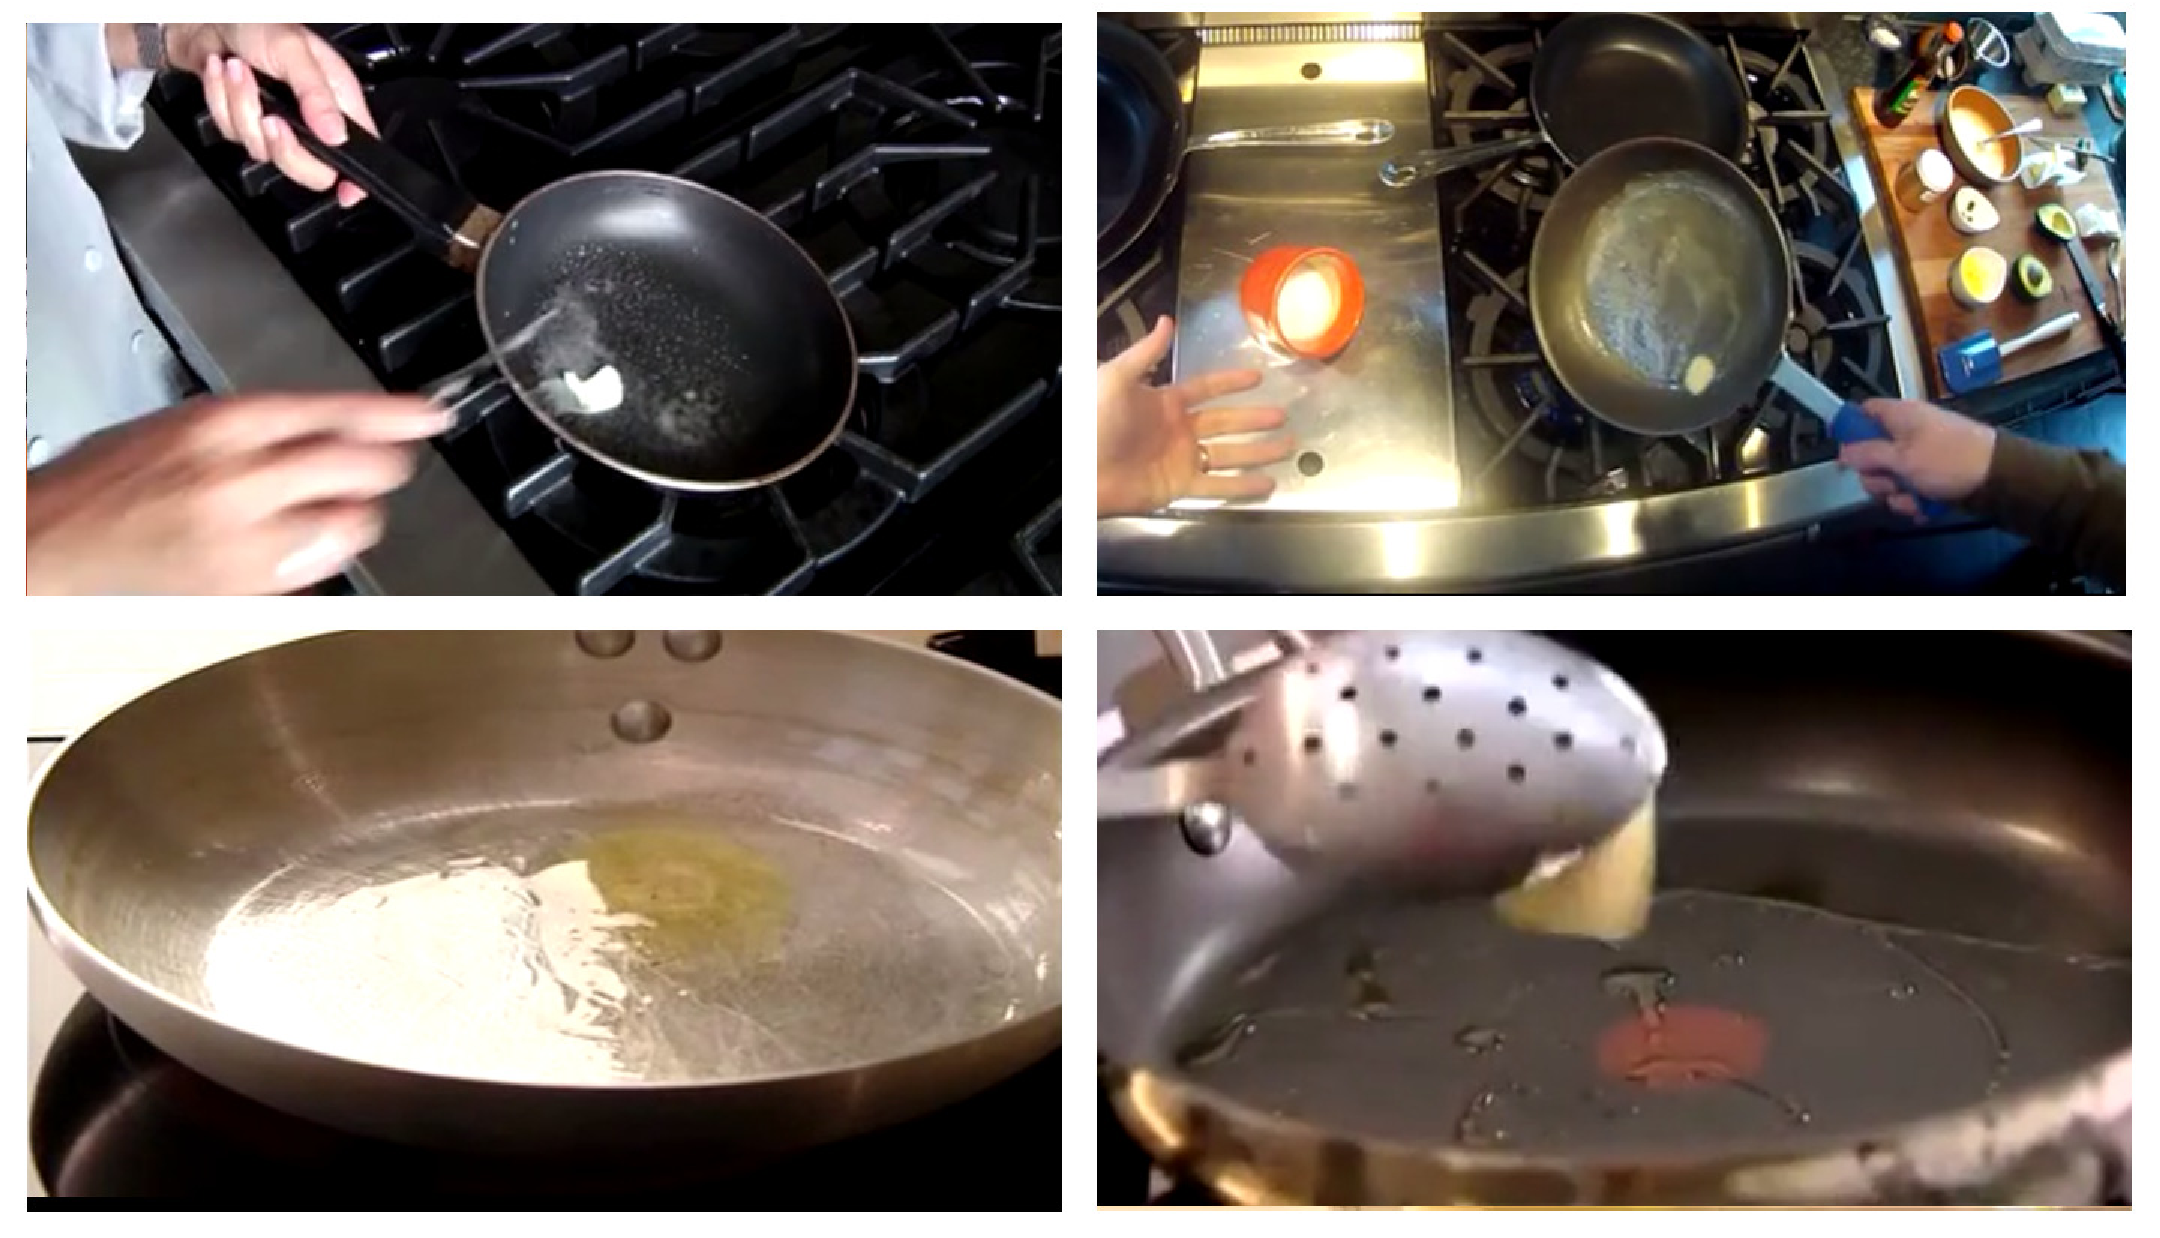
\includegraphics[width=\textwidth]{cgreen}
\color[HTML]{9DFF00}{Eggs cook quickly, so make sure the pan gets very hot first; the butter melt completely.}
\end{subfigure}
\caption{Temporal segmentation of the videos by our method and ground truth segmentation. We also color code the learned activity labels and visualize sample frames and the automatically generated captions for some of them. \emph{Best viewed in color.}}
\label{recipe:ommelette}
\fi
%\normalsize}
\end{figure*}

As shown in the Figures~\ref{recipe:ommelette}\&\ref{recipe:milkshake}, resulting clusters are semantically meaningful and correspond to the real activities. Moreover, sthe language captions are also quite informative hence we can conclude that there is enough language context within the subtitles in order to detect activities. On the other hand, some of the activities in the ground truth are not detected by our algorithm and they got merged into other clusters because they generally occur only in a very few videos.
\subsection{Quantitative Results}
\begin{figure*}[t]
  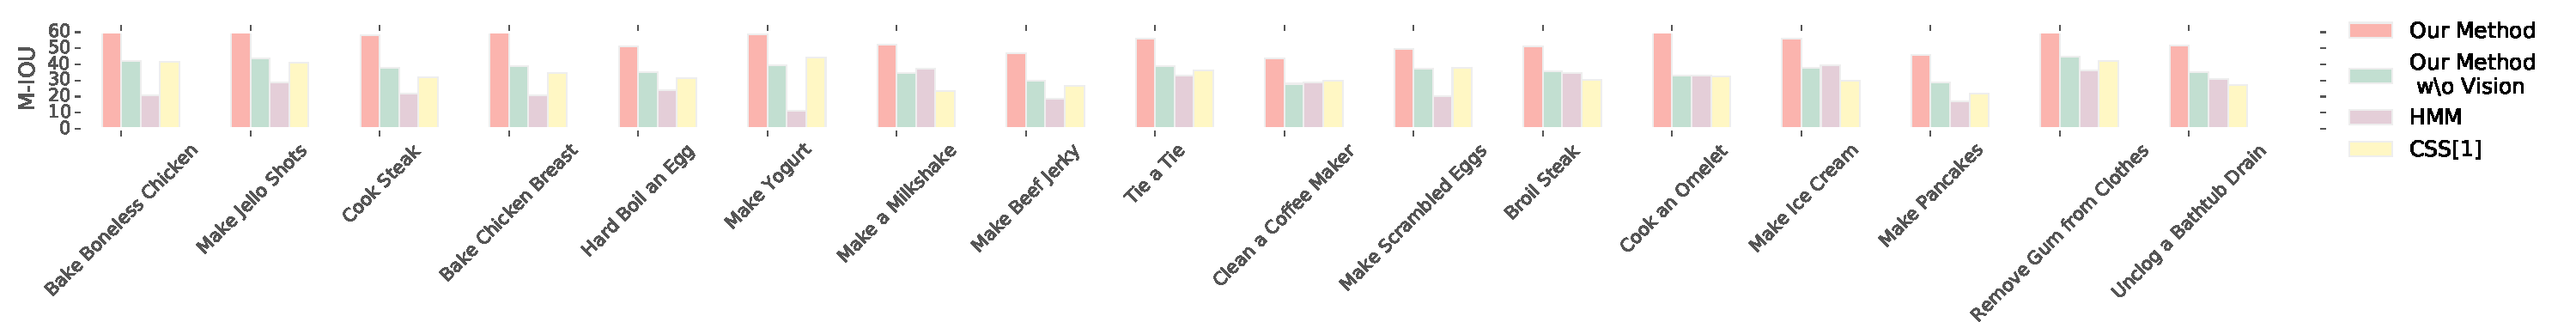
\includegraphics[width=\textwidth]{miou}
  \caption{$IOU_{max}$ stuff, not real numbers just a place holder}
  \label{mIOU}
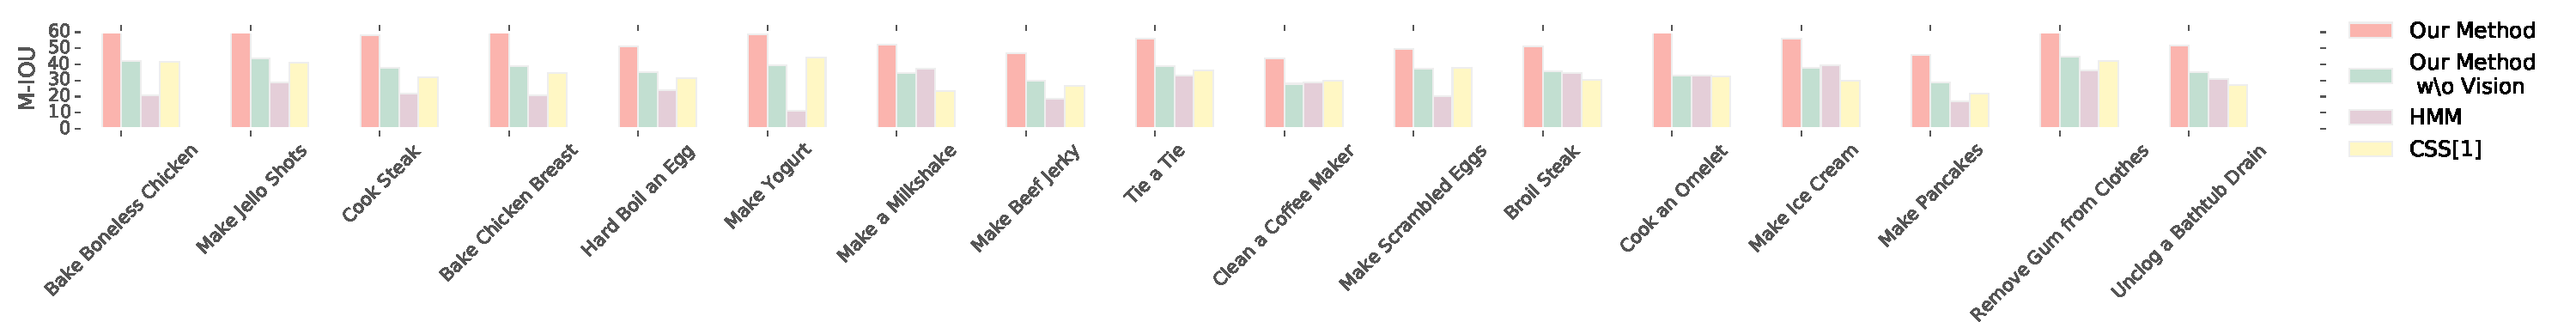
\includegraphics[width=\textwidth]{miou}
\caption{$AP_{max}$ stuff, not real numbers just a place holder}
\label{mmAP}
\end{figure*}

\subsubsection{Baselines}
We compare our algorithm with the following baselines in the following sections.

\noindent\textbf{HMM with semantic features:}
In order to experiment the importance of joint processing of the videos, we compare our algorithm with independent temporally coherent clustering of each video. We are using Hidden Markov Models with Baum-Welch algorithm\cite{rabiner} as a clustering method and choose the number of clusters with cross-validation.

\noindent\textbf{BP-HMM with low-level features:}
In order to experiment the importance of defining objects, we also train our algorithm without using extracted object. We simply temporally oversegment the video and represent each segment by using state of the art low-level features from the activity detection literature \cite{acticityFeature}. We are using dense trajectory features for this purpose.

\noindent\textbf{Category specific summary\cite{potapov2014category}:}
An algorithm porposed by Potapov et al.\cite{potapov2014category} can detect the temporal boundaries of the events/activities in the video from a time series data without any supervision. It enforces a local similarity of each resultant segment.

\subsubsection{Metrics}
\noindent\textbf{Maximum Intersection over Union ($IOU_{max}$):}
In order to evaluate the accuracy of the temporal segmentation of the activities, we use intersection-over-union(IOU). For $N$ ground truth temporal activity segments ($\tau^\star_{i},\quad i\in N$), $N^\prime$ computed segments ($\tau^\prime_{i},\quad i\in N^\prime$) and matching function $m(\cdot)$ such that $i^{th}$ ground truth segment is matched to $m(i)^{th}$ computed segment, we define IOU as \mbox{$IOU=\frac{1}{N}\sum_{i=1}^N \frac{\tau^\star_i \cap \tau^\prime_{m(i)}}{\tau^\star_i \cup \tau^\prime_{m(i)}}$}. Since the matching function is unknown in thte supervised setting, we use the maximum intersection-over-union while doing exhaustive search over all matchings as;
\mbox{$IOU_{max} = \max_{m(\cdot)} \frac{1}{N}\sum_{i=1}^N \frac{\tau^\star_i \cap \tau^\prime_{m(i)}}{\tau^\star_i \cup \tau^\prime_{m(i)}}$}

\noindent\textbf{Maximum Average Precision ($AP_{max}$):}
Since the $IOU_{max}$ is computed per video, it does not capture the accuracy of the detected activities over multiple videos. Hence, we also evaluate maximum average precision. Given matching function $m(\cdot)$, the average precision is defined as $\frac{1}{N}\sum_{i =1}^N\frac{tp_i}{tp_i+fp_i}$ where $tp_i$ is the number of frames correctly labeled with activity $i$ and $fp$ is the number of frames falsely labelled as activity $i$. Note that this metric is defined over all the videos in the recipe and can only be high if the the same activities from multiple videos clustered into a single activity. Similarly, the maximum is over matching functions as \mbox{$AP_{max}=\max_{m(\cdot)} \frac{1}{N}\sum_{i =1}^N\frac{tp_i}{tp_i+fp_i}$} 

%\noindent\paragraph{Semantic Correctness:}

\subsubsection{Results}
We discuss the quantitative and qualitative results in the light of the following questions.
\paragraph{Are the activities detected accurately?}
In this section, we discuss the results presented in Figure~\ref{mIOU}. Maximum-IOU captures the accuracy of the temporal segmentation of the videos. Since the ground-truth segmentation is the semantic one, high $IOU_{max}$ requires both finding temporal activity boundaries and extracting correct activity definition. As shown in the Figure~\ref{mIOU}, proposed method consistently outperforms the competing algorithms. One interesting observation is the dramatic difference between the accuracy of HMM and our method. We believe this is the result of joint processing of multiple videos. HMM assumes all videos are generated from same set of activities with fixed transition probabilities and can not captures the inter-class variance. On the other hand, our algorithm is roboust to inter-class variations since we are also modelling inclusion of activities for each video. Moreover, the segmentation problem is ill-posed since the granularity of the activities are subjective. Imposing the activity inclusion model brings an additional constraint to the problem and makes the problem well-posed as finding the set of small number of activities which can construct the any video within the context of the recipe. In other words, the segmentation problem becomes learning the small dictionary of activities which is complete for the space of the recipe.

\paragraph{Are the same activities in different videos linked to each other?}
Although $IOU_{max}$ successfully measures the accuracy of the detected activities, it can not measure the matching activities over different videos. Therefore, we are using $AP_{max}$ for measuring the accuracy of matching different activities over multiple videos. $AP_{max}$ is defined for each activity class and requires the algorithms to produce activity labels consistent with the ground truth. 
%\paragraph{Semantics vs Syntax:} Should we do the extra experiments, dow we have time?
\paragraph{How important is each modality?}
In order to experiment the importance of using both language and vision modalities, we compare our method with a self-baseline of using a single modality. As shown in Figure~\ref{mIOU} and \ref{mmAP}, our method significantly outperforms both of the baselines consistently in all recipes. Hence, we need to use both modalities. This result is expected because visual cues are good at separating different activities within the same video since the visual appearance is not changing much. However, language does not help much since there is too much background information other than the actual activity. On the other hand, language is good at relating activities from different videos since there is not much inter-class variation and it is easy to detect these variations caused by synonyms etc. thanks to the strong structure of the language modality.
